\documentclass{article}
\usepackage[utf8]{inputenc}
\usepackage{lipsum} % Paquete para generar texto de prueba
\usepackage{graphicx} % Para incluir imágenes
\usepackage{tikz} % Para dibujar figuras

\usepackage{geometry} % Para ajustar el tamaño del texto y los márgenes
% Ajusta el tamaño del texto y los márgenes
\geometry{
    left=30mm, % Margen izquierdo
    top=25mm, % Margen superior
}
\usepackage{float} % Para la opción [H]
\usepackage{enumitem}
\usepackage[spanish]{babel} % Cargar el idioma español

\usepackage{listings}

 % Configuración del estilo de las celdas de código
\lstset{
  frame=single, % Agrega un marco alrededor del código
  language=Python, % Lenguaje del código
  basicstyle=\ttfamily\small, % Estilo básico del texto del código
  keywordstyle=\color{blue}, % Estilo de las palabras clave
  commentstyle=\color{green!40!black}, % Estilo de los comentarios
  stringstyle=\color{red}, % Estilo de las cadenas de texto
  showstringspaces=false, % No mostrar espacios en cadenas de texto
  captionpos=b, % Posición de la leyenda (abajo)
}

\usepackage{hyperref}

\title{\textbf{SINCRONIZACION CAMARAS}\\[0.5em] \large Investigacion UHPC}
\author{Lukas Wolff Casanova}
\date{\today}
\begin{document}

\maketitle
\hrule

\section{INTRODUCCION}

\noindent Actualmente se está utilizando el método PIV en la simulación del carbopol, el cual, en pocas palabras, utiliza un plano bidimensional para rastrear partículas. El problema radica en que buscamos hacer la simulación en torno a fibras, las cuales pueden rotar, por lo cual es necesario implementar una simulación tridimensional para poder utilizar la tecnología PTV.
\\ \\
En base a lo anterior, se plantea lograr una sincronización de las cámaras para así poder implementar el software.

\section{METODOLOGIA}

\noindent Para poder realizar una sincronización de las cámaras es necesario implementar un trigger, el cual puede ser mediante software (SW) o hardware (HW). Previo a decidir cuál era el trigger correcto a implementar, se comenzó a armar el setup para poder sincronizar las cámaras.
\\ \\
El setup consistió básicamente de una hélice sobre un motor brushless, donde, mediante un sensor infrarrojo, se podía medir sus revoluciones en tiempo real. Además, se diseñó un soporte para las cámaras, de modo que estas estuvieran alineadas en todo momento.
\\ \\
Los diseños 3D realizados son los siguientes:

\begin{figure}[H]
    \centering
    \begin{minipage}[b]{0.3\textwidth}
      \centering
      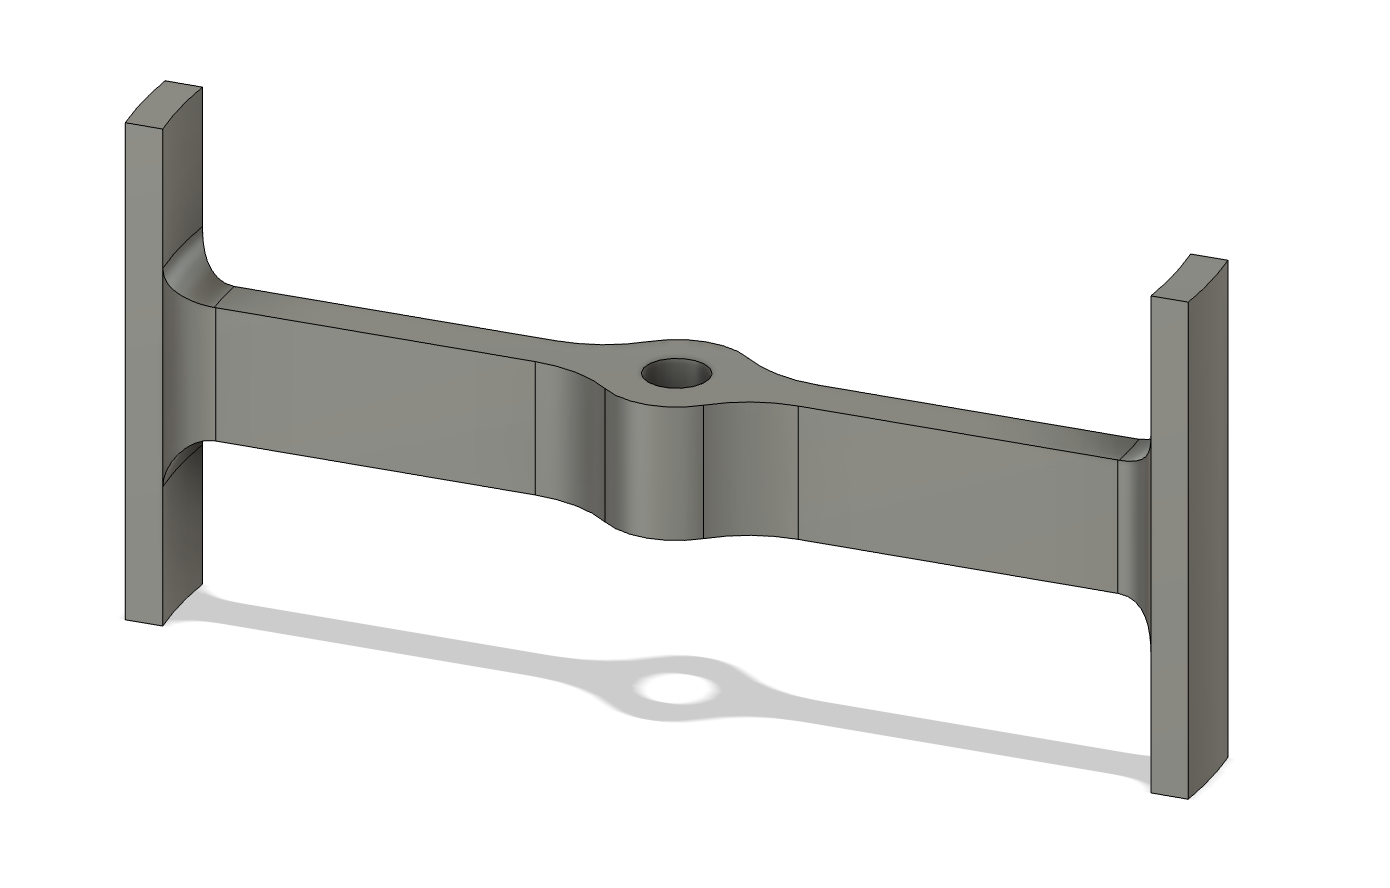
\includegraphics[width=\textwidth]{MODELOS/HELICE.png}
      \caption{Helice}
    \end{minipage}
    \begin{minipage}[b]{0.3\textwidth}
      \centering
      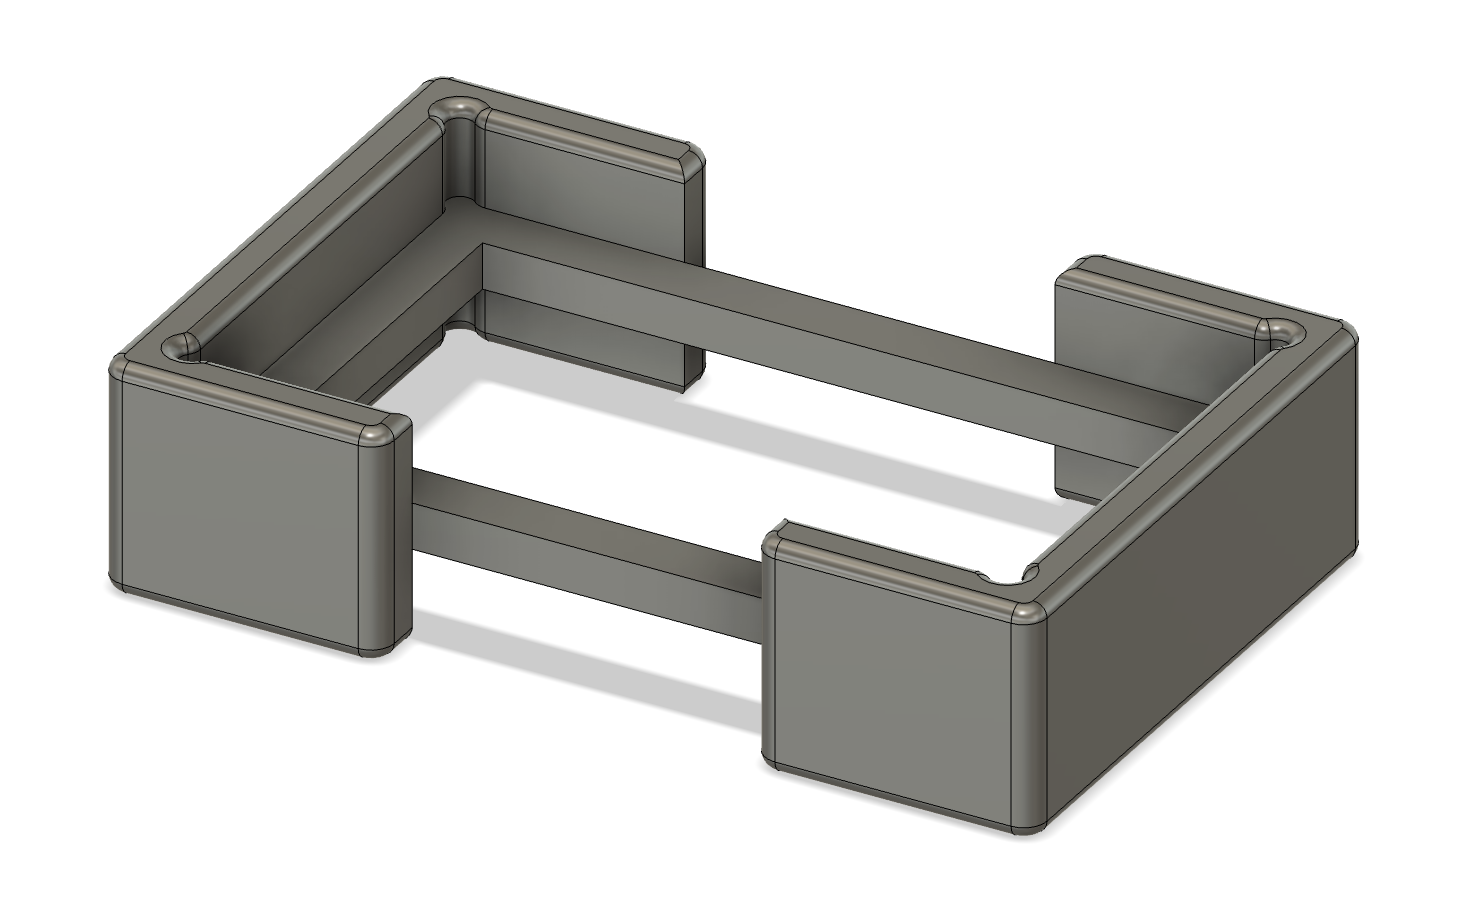
\includegraphics[width=\textwidth]{MODELOS/CAMARAS.png}
      \caption{Soporte camaras}
    \end{minipage}
    \begin{minipage}[b]{0.3\textwidth}
      \centering
      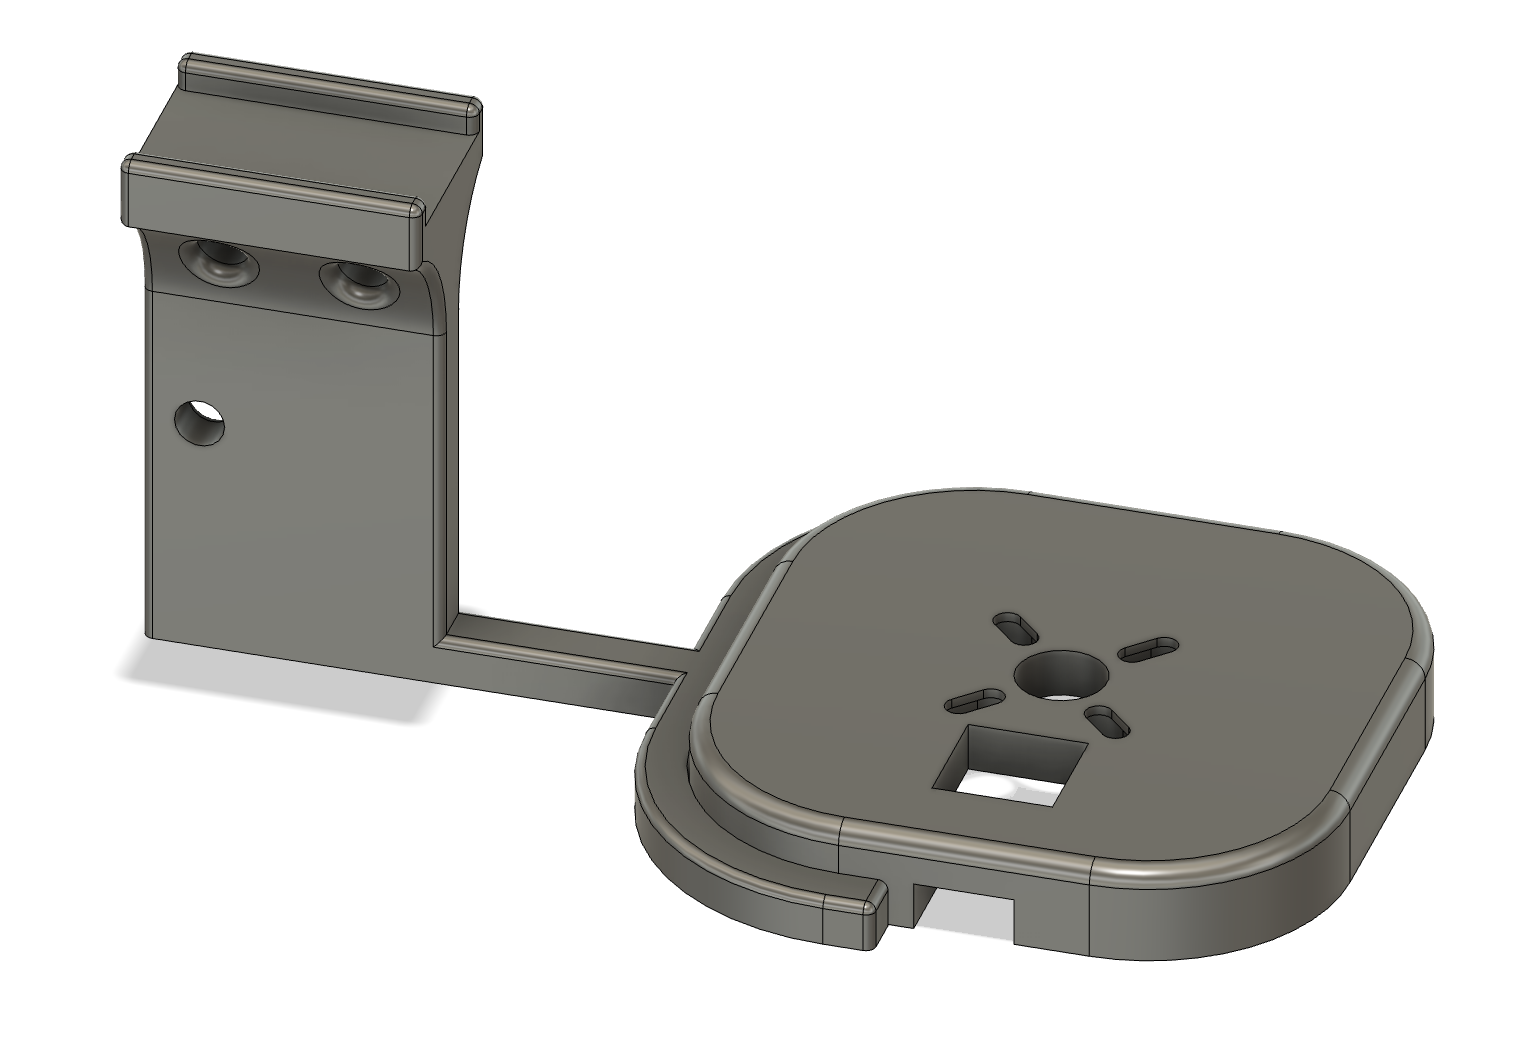
\includegraphics[width=\textwidth]{MODELOS/MOTOR.png}
      \caption{Soporte motor y sensor}
    \end{minipage}
\end{figure}

\newpage
\noindent A continuación se mostrarán las iteraciones para llegar al setup final.

\begin{figure}[H]
    \centering
    \begin{minipage}[c]{0.25\textwidth}
      \centering
      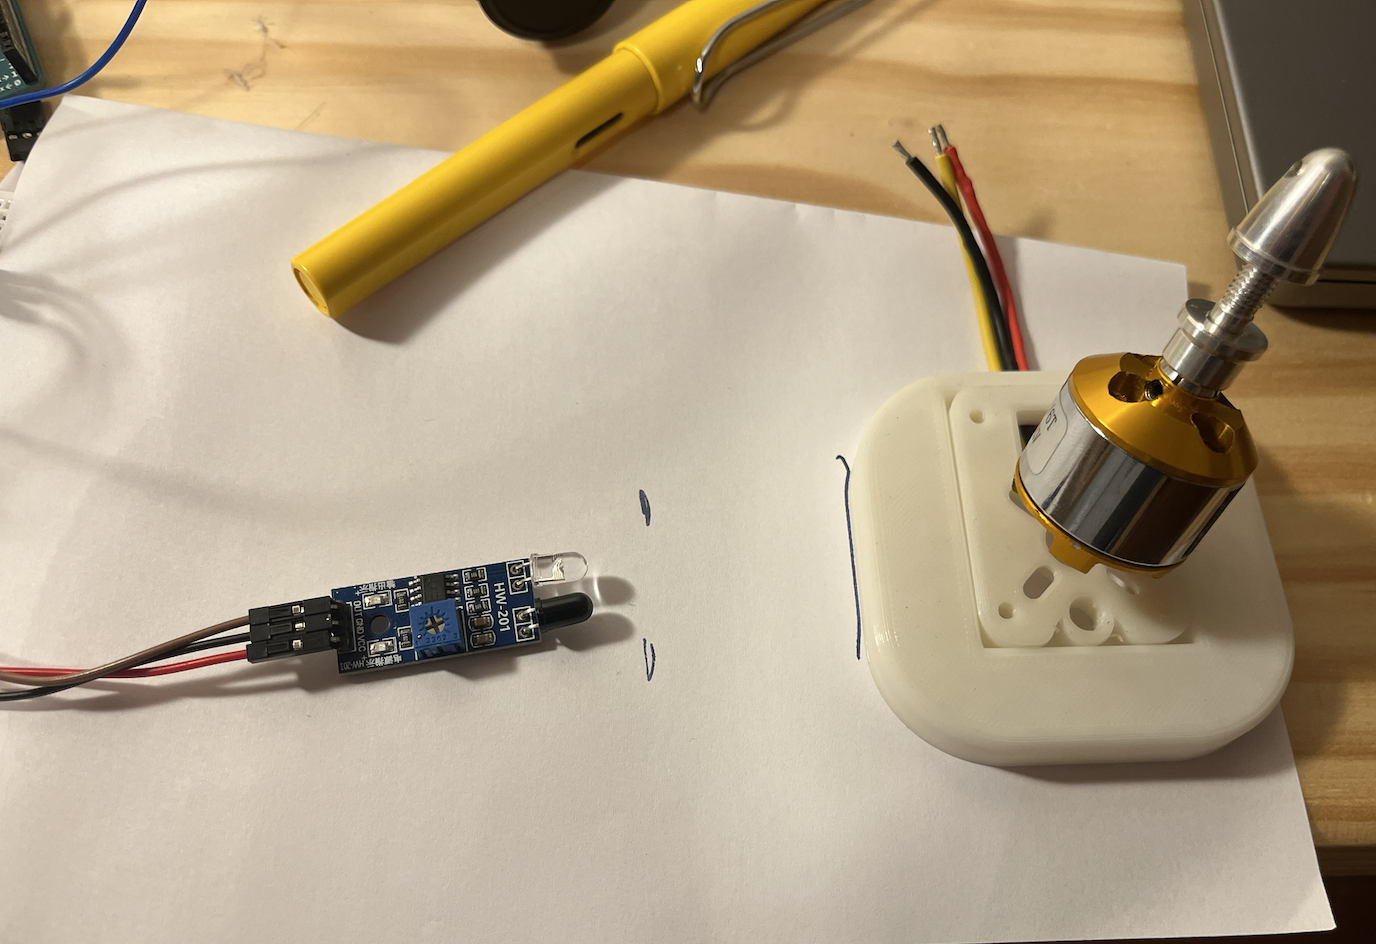
\includegraphics[width=\textwidth]{FOTOS/PS.png}
      \caption{Prueba sensor}
    \end{minipage}
    \begin{minipage}[c]{0.25\textwidth}
      \centering
      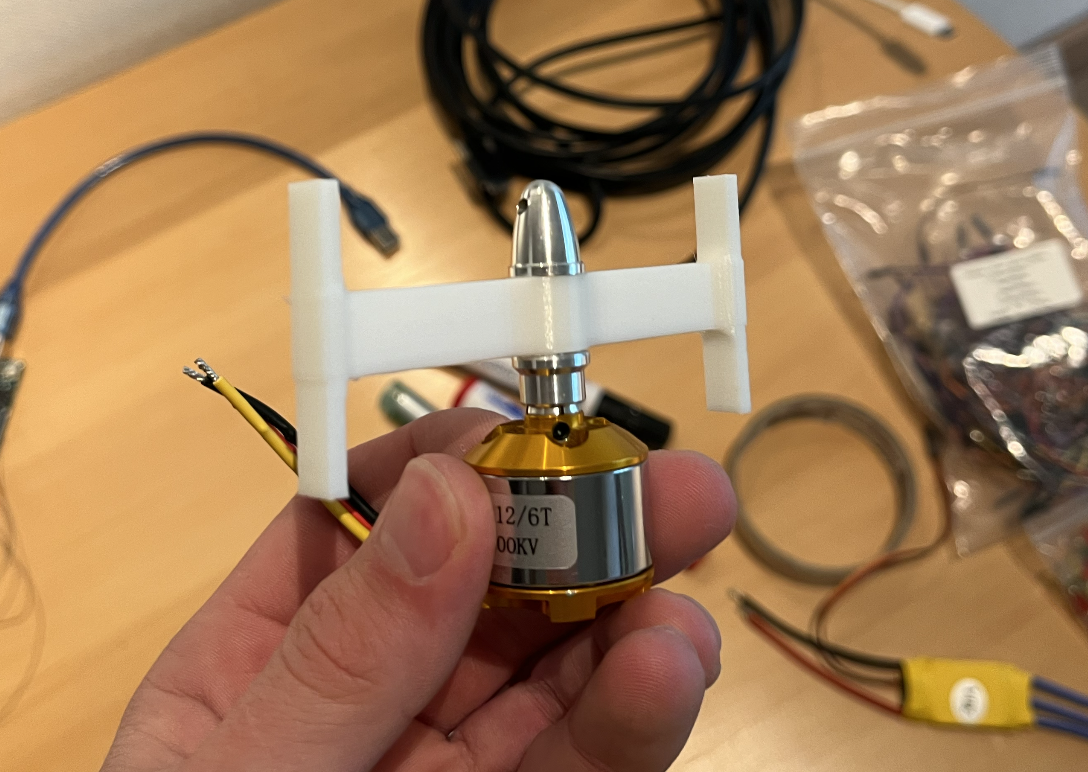
\includegraphics[width=\textwidth]{FOTOS/H.png}
      \caption{Helice}
    \end{minipage}
    \begin{minipage}[c]{0.25\textwidth}
      \centering
      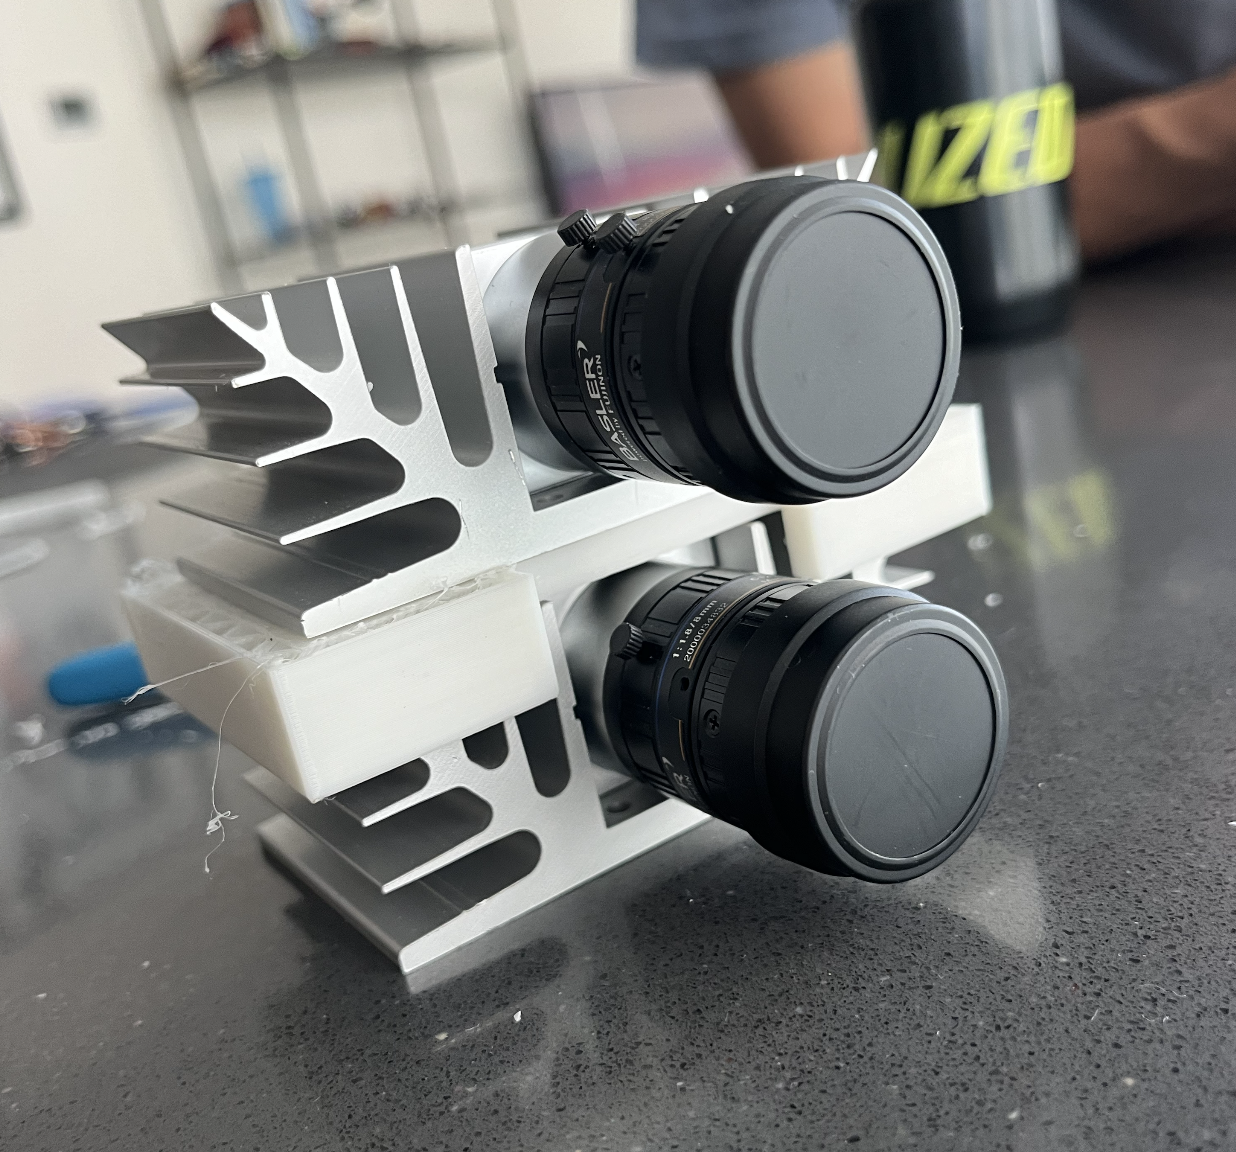
\includegraphics[width=\textwidth]{FOTOS/C.png}
      \caption{Prueba soporte camaras}
    \end{minipage}
\end{figure}

\noindent Se determinó que el sensor infrarrojo no lograba medir correctamente las revoluciones, ya que este utilizaba el reflejo de la luz y no alcanzaba a recibir la señal de vuelta. El profesor Jorge sugirió utilizar un medidor de revoluciones láser.
\\ \\
Al mismo tiempo que se realizaba el setup, se contactó a Basler, quienes nos redirigieron con un contacto en Chile. Hablando con Jorge (el contacto), se concluyó que la mejor forma de realizar el trigger es mediante software, donde además nos dio un hub de Python como guía.
\\ \\
El código Python se optimizó de modo que durante el ciclo de fotos, estas solo se guardan en una variable sin procesar, y posteriormente, se almacenan como imágenes visibles y no como un array.
\\ \\
Finalmente, el setup es el siguiente:

\begin{figure}[H]
    \centering
    \begin{minipage}[c]{0.3\textwidth}
      \centering
      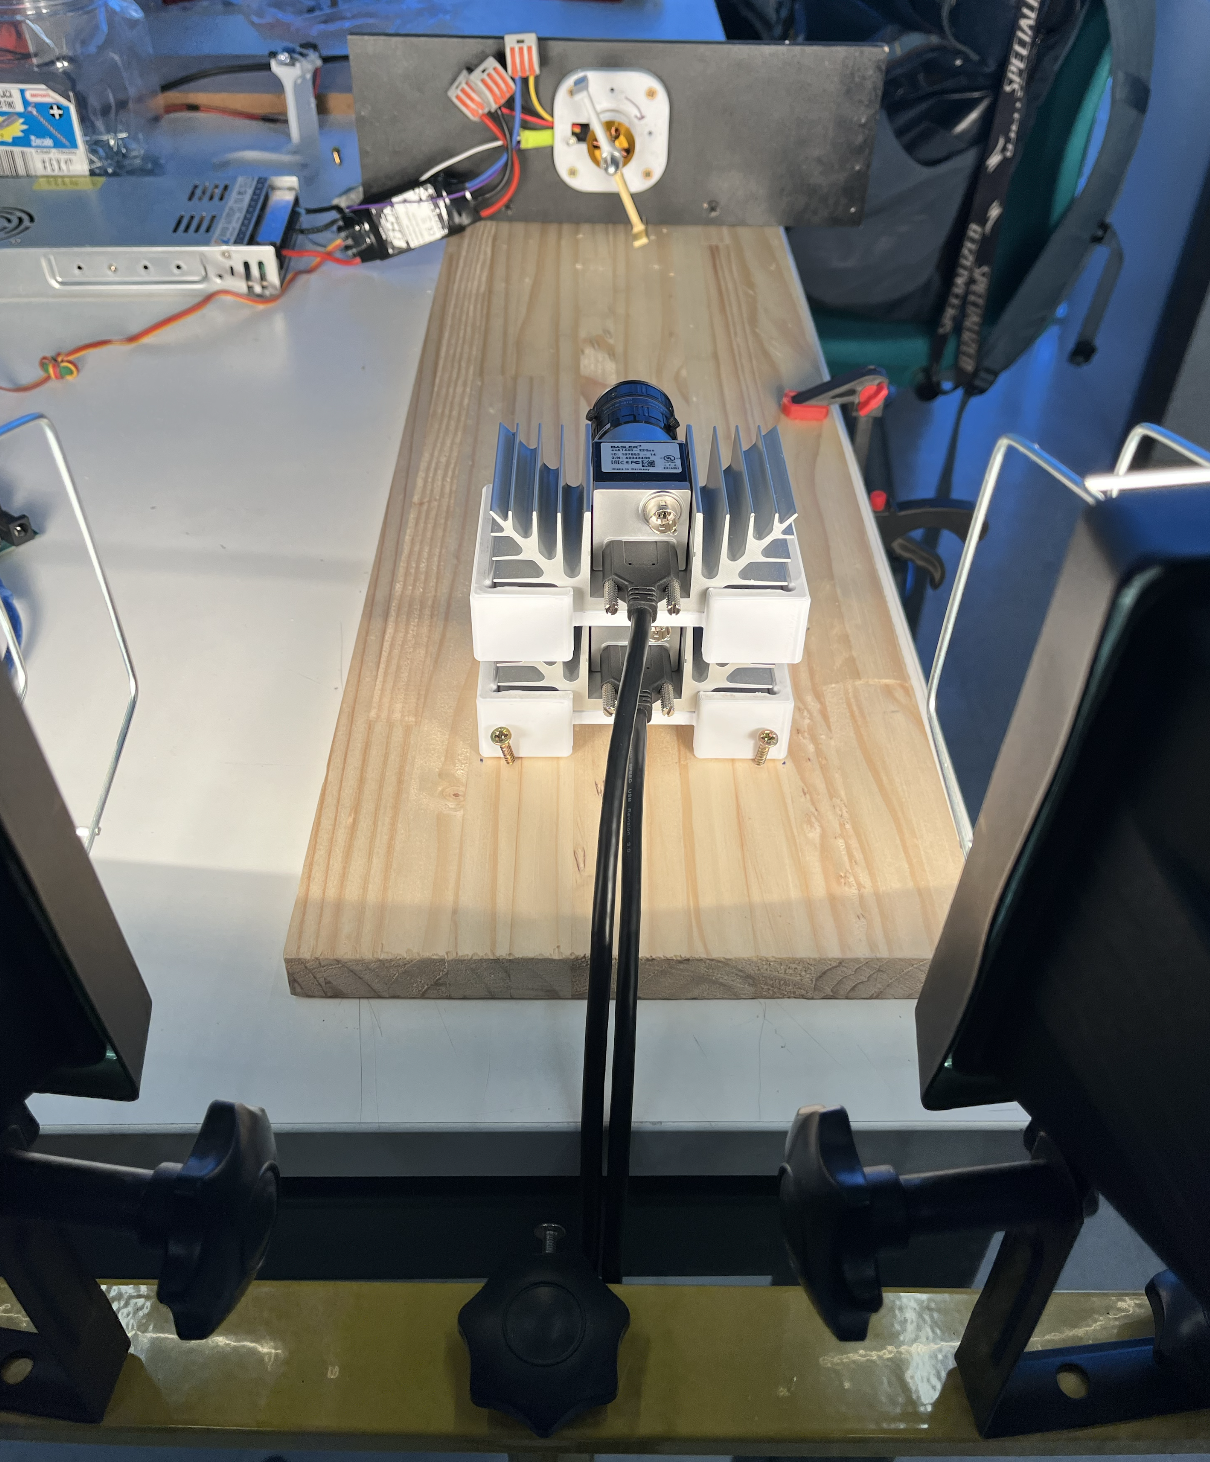
\includegraphics[width=\textwidth]{FOTOS/SF.png}
      \caption{Setup final 1}
    \end{minipage}
    \begin{minipage}[c]{0.3\textwidth}
      \centering
      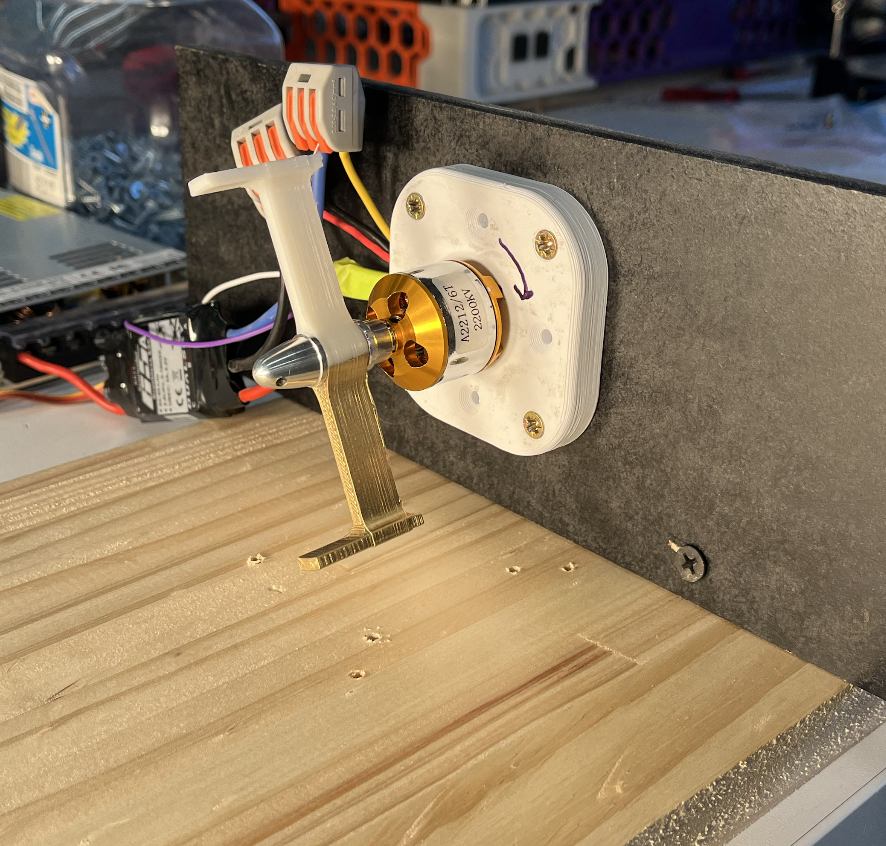
\includegraphics[width=\textwidth]{FOTOS/HF.png}
      \caption{Setup final 2}
    \end{minipage}
\end{figure}

\noindent Por lo tanto, el proceso para realizar una medición es el siguiente:

\begin{itemize}
    \item Encender motor brushless
    \item Medir RPM
    \item Disparar cámaras
\end{itemize}

\noindent Es importante notar que el motor gira en sentido horario. Además, las mediciones fueron realizadas a 200 FPS.

\newpage
\section{RESULTADOS}

\noindent A continuación se mostrarán las fotos de una medición a 5645 RPM.

\begin{figure}[H]
    \centering
    \begin{minipage}[b]{0.45\textwidth}
      \centering
      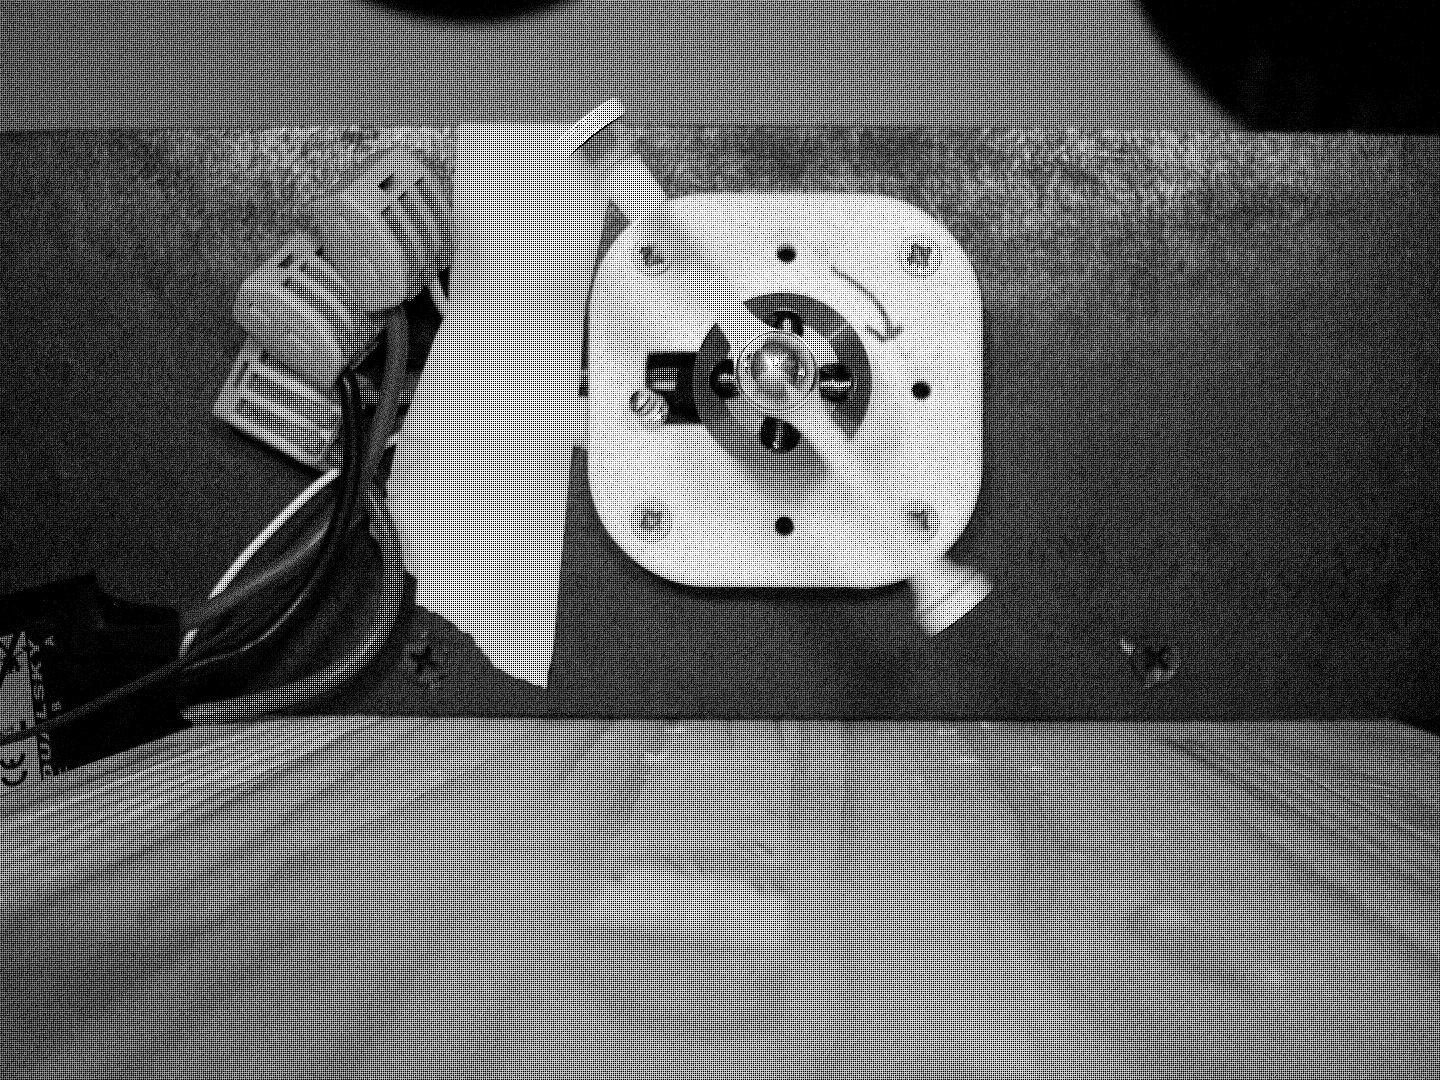
\includegraphics[width=0.8
      \textwidth]{FOTOS_C/5645/0/1.png}
      \caption{Imagen 1 camara 0}
    \end{minipage}
    \begin{minipage}[b]{0.45\textwidth}
      \centering
      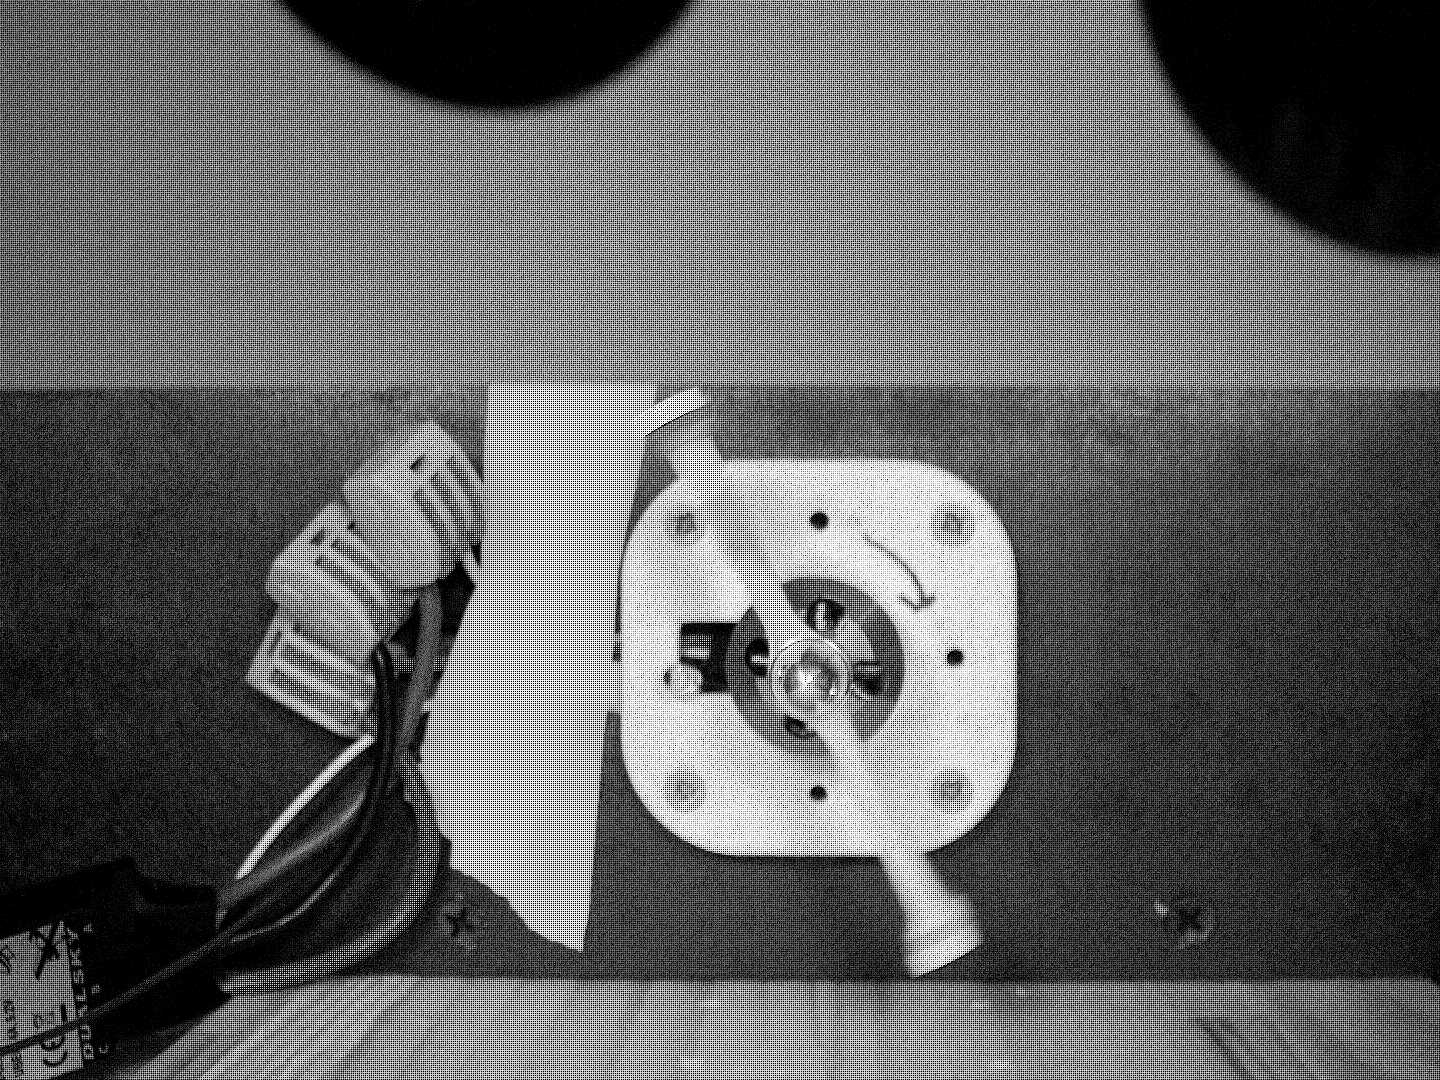
\includegraphics[width=0.8
      \textwidth]{FOTOS_C/5645/1/1.png}
      \caption{Imagen 1 camara 1}
    \end{minipage}
    \begin{minipage}[b]{0.45\textwidth}
      \centering
      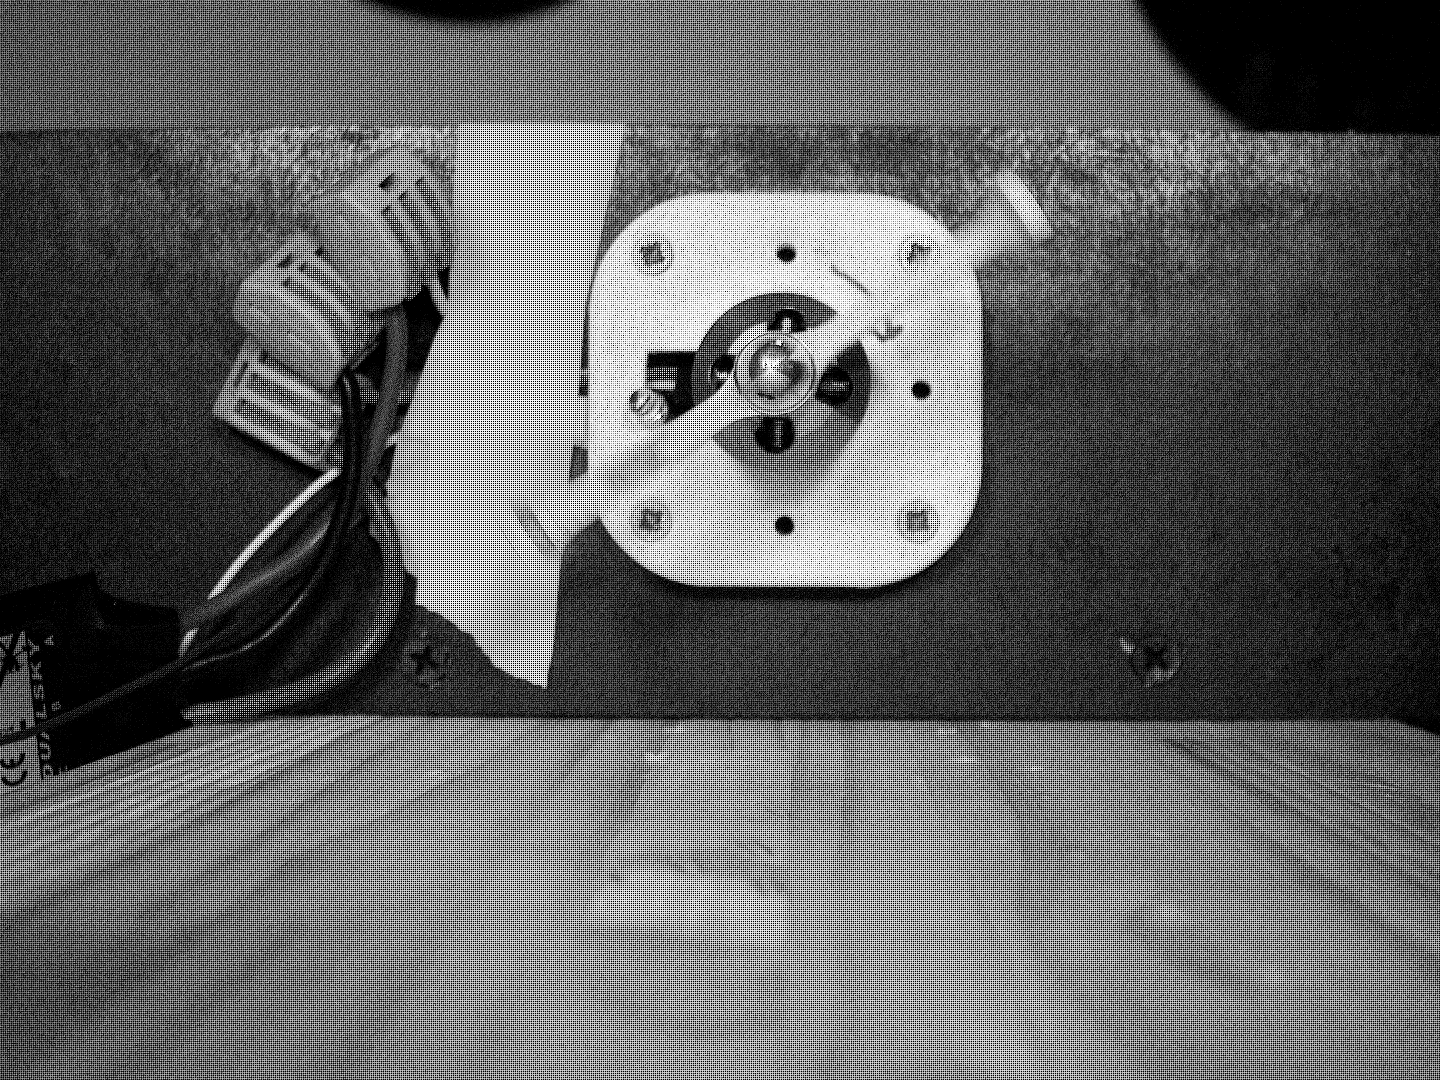
\includegraphics[width=0.8
      \textwidth]{FOTOS_C/5645/0/2.png}
      \caption{Imagen 2 camara 0}
    \end{minipage}
    \begin{minipage}[b]{0.45\textwidth}
      \centering
      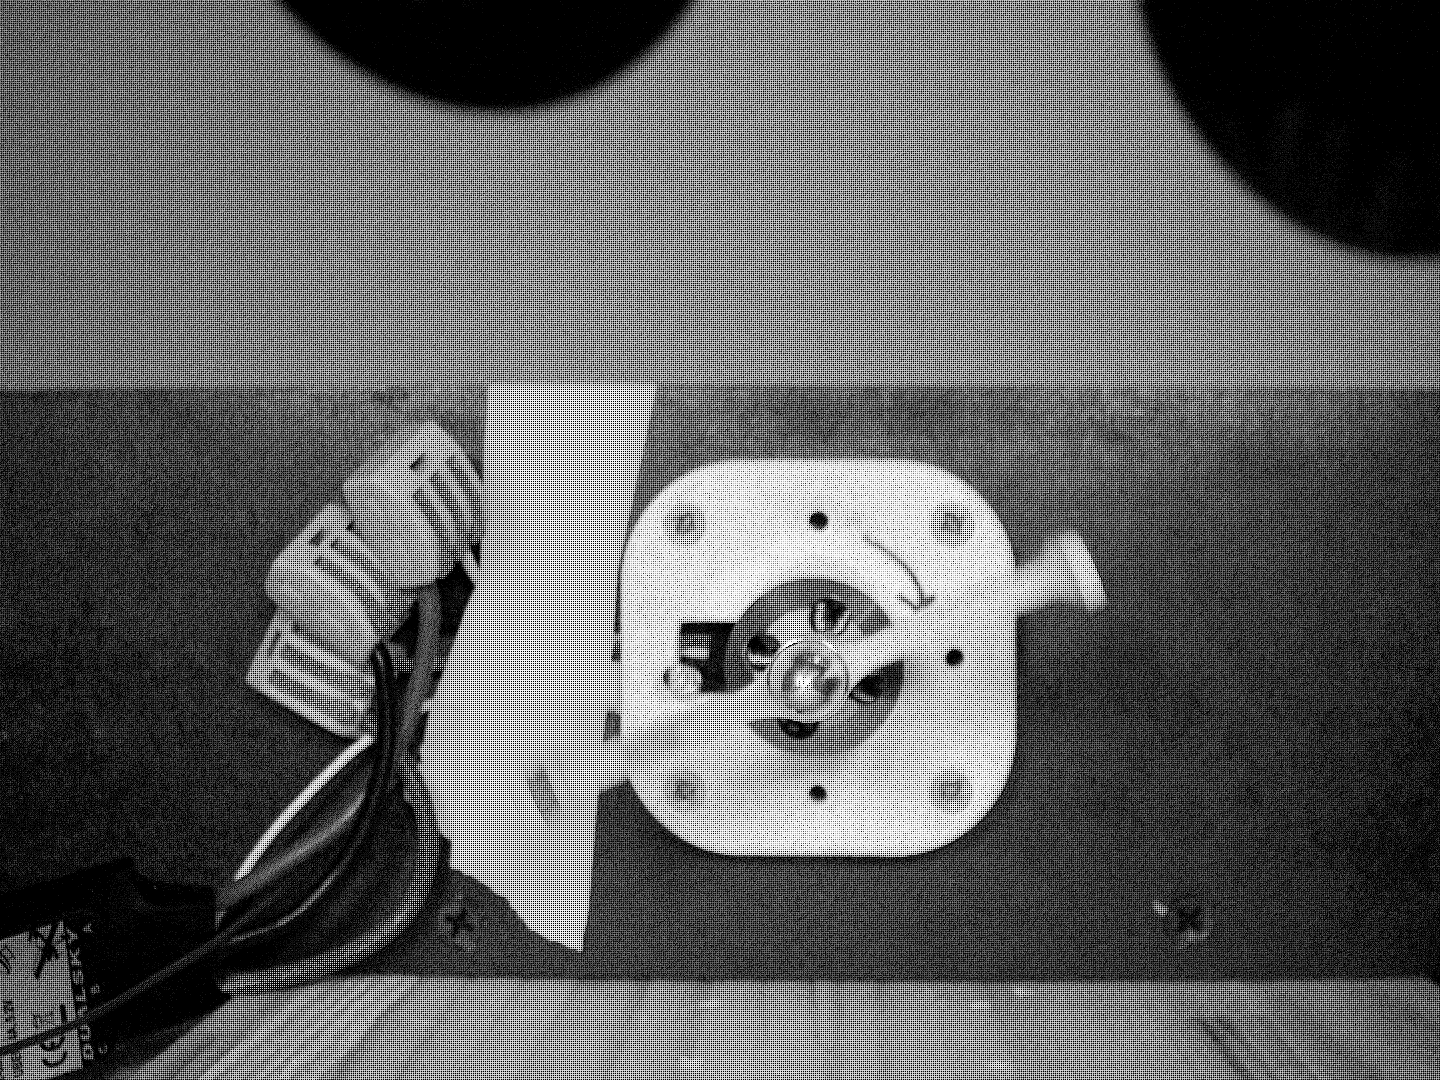
\includegraphics[width=0.8
      \textwidth]{FOTOS_C/5645/1/2.png}
      \caption{Imagen 2 camara 1}
    \end{minipage}
    \begin{minipage}[b]{0.45\textwidth}
      \centering
      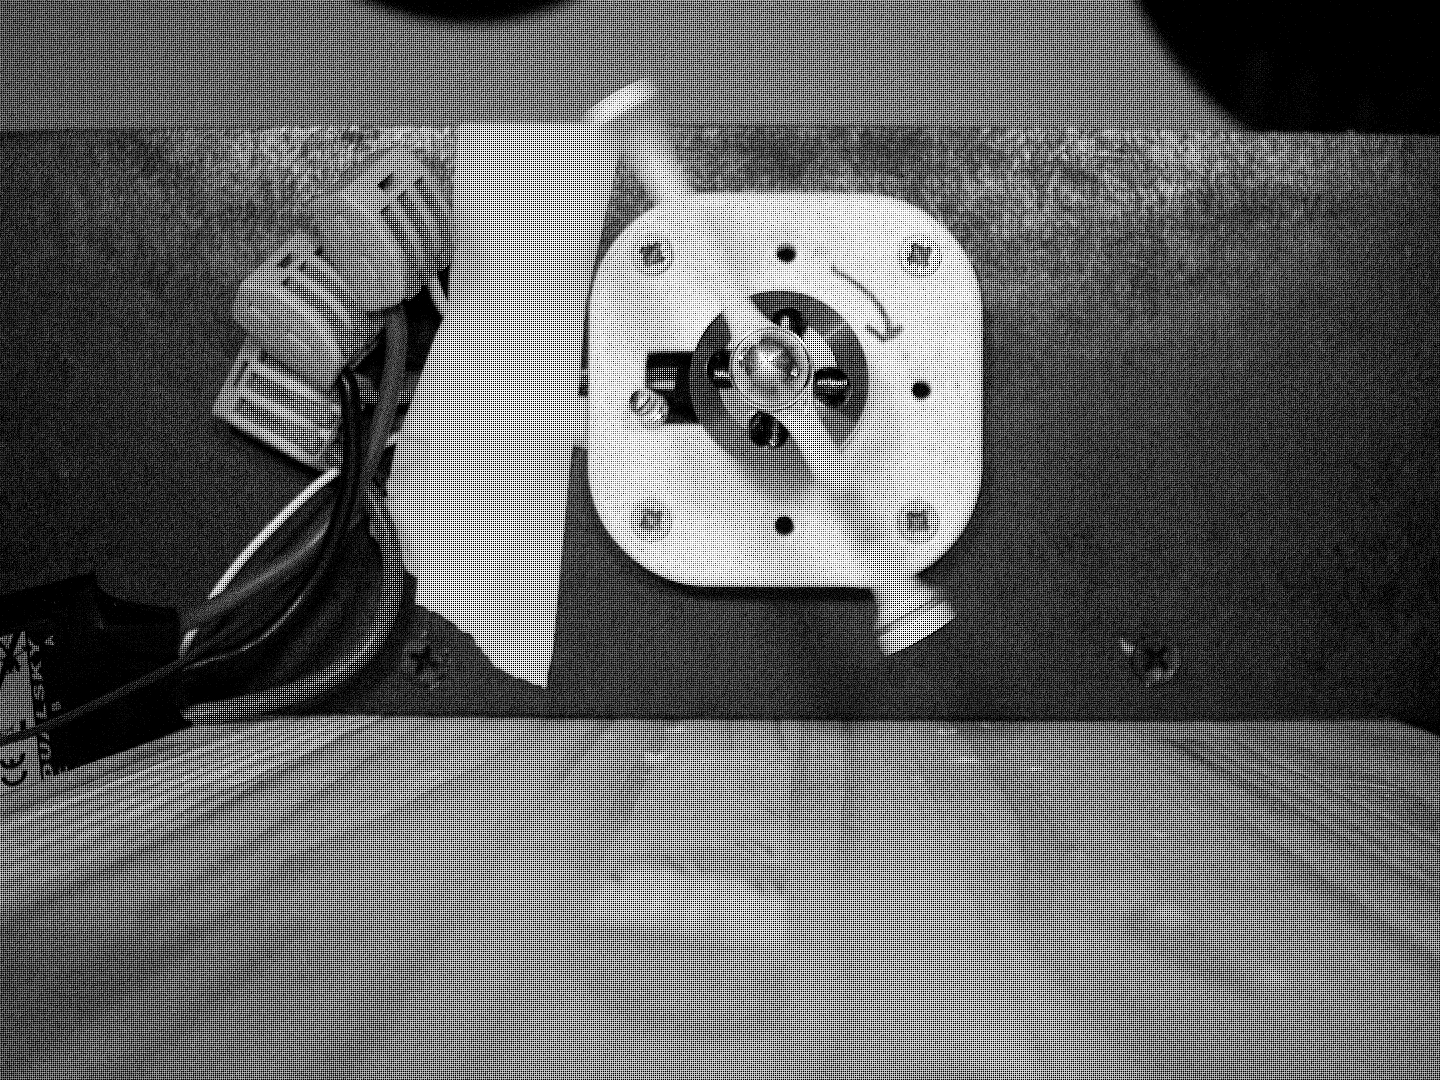
\includegraphics[width=0.8
      \textwidth]{FOTOS_C/5645/0/3.png}
      \caption{Imagen 3 camara 0}
    \end{minipage}
    \begin{minipage}[b]{0.45\textwidth}
      \centering
      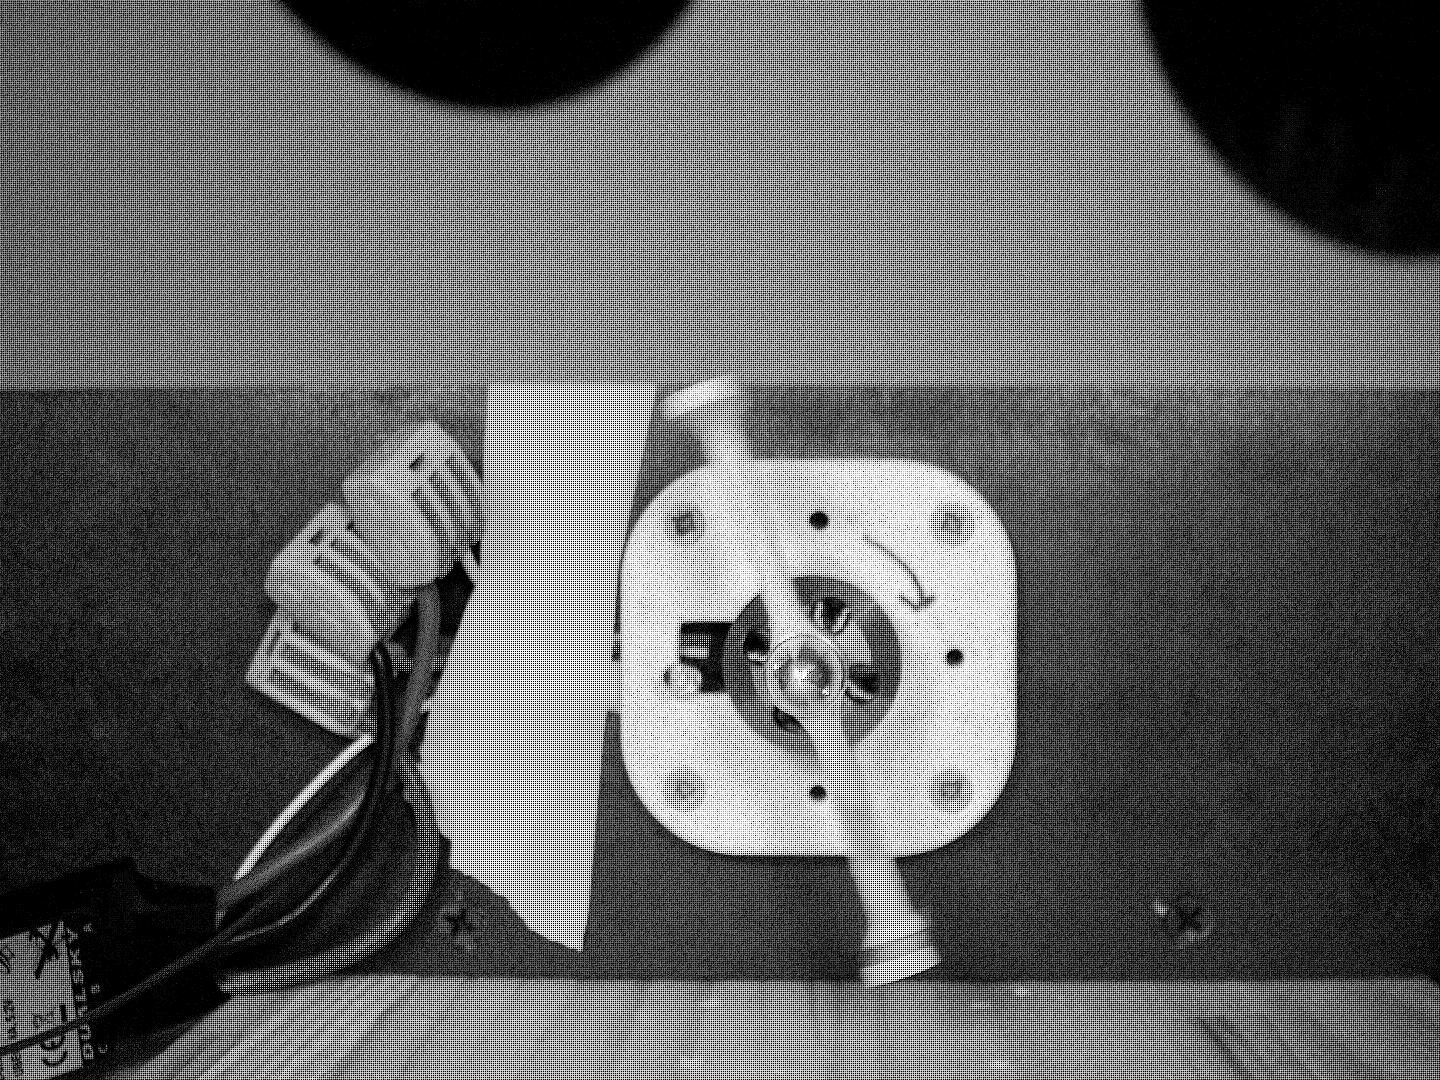
\includegraphics[width=0.8
      \textwidth]{FOTOS_C/5645/1/3.png}
      \caption{Imagen 3 camara 1}
    \end{minipage}
    \begin{minipage}[b]{0.45\textwidth}
      \centering
      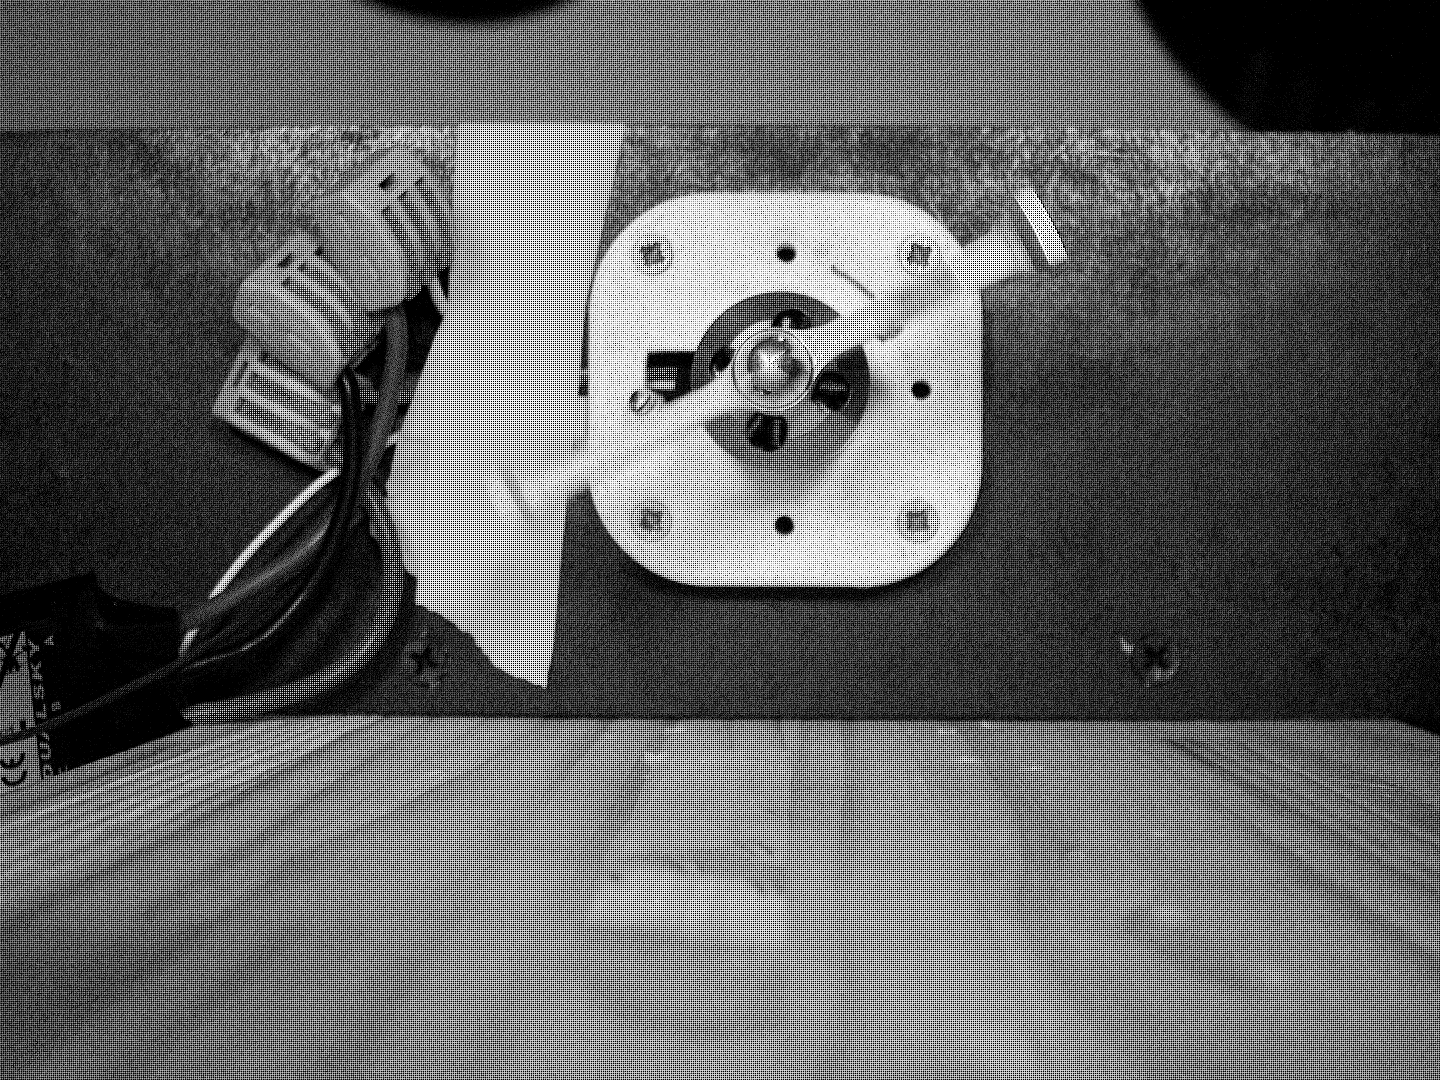
\includegraphics[width=0.8
      \textwidth]{FOTOS_C/5645/0/4.png}
      \caption{Imagen 4 camara 0}
    \end{minipage}
    \begin{minipage}[b]{0.45\textwidth}
      \centering
      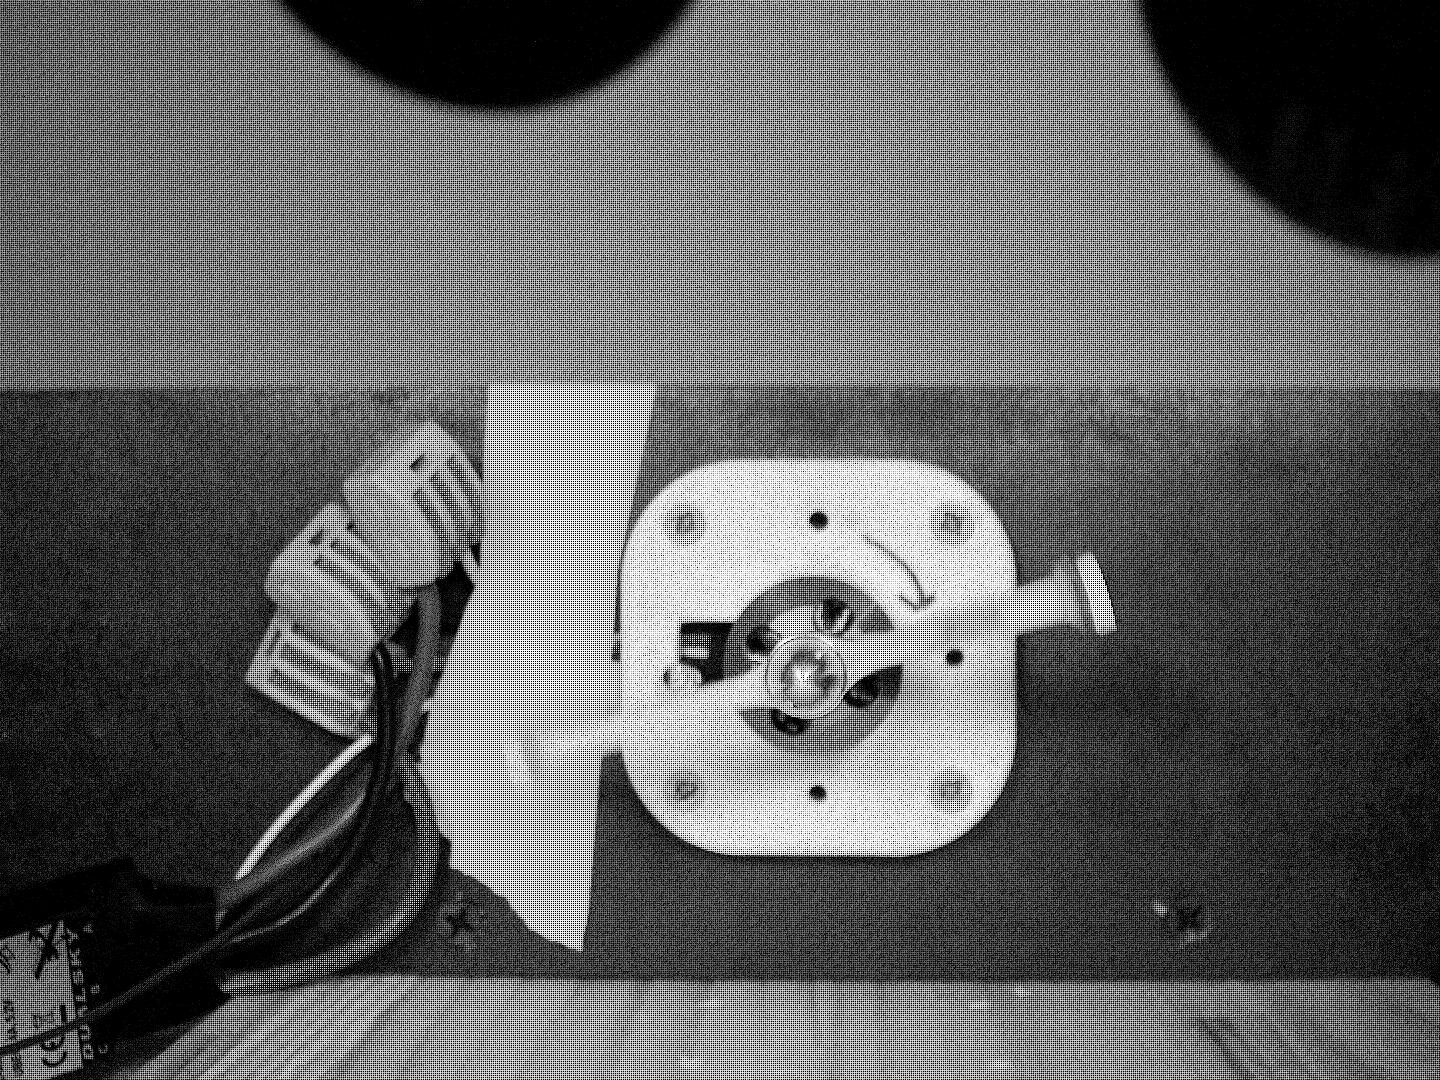
\includegraphics[width=0.8
      \textwidth]{FOTOS_C/5645/1/4.png}
      \caption{Imagen 4 camara 1}
    \end{minipage}
\end{figure}

\newpage
\noindent A continuación se mostrarán las fotos de una medición a 8519 RPM.

\begin{figure}[H]
    \centering
    \begin{minipage}[b]{0.45\textwidth}
      \centering
      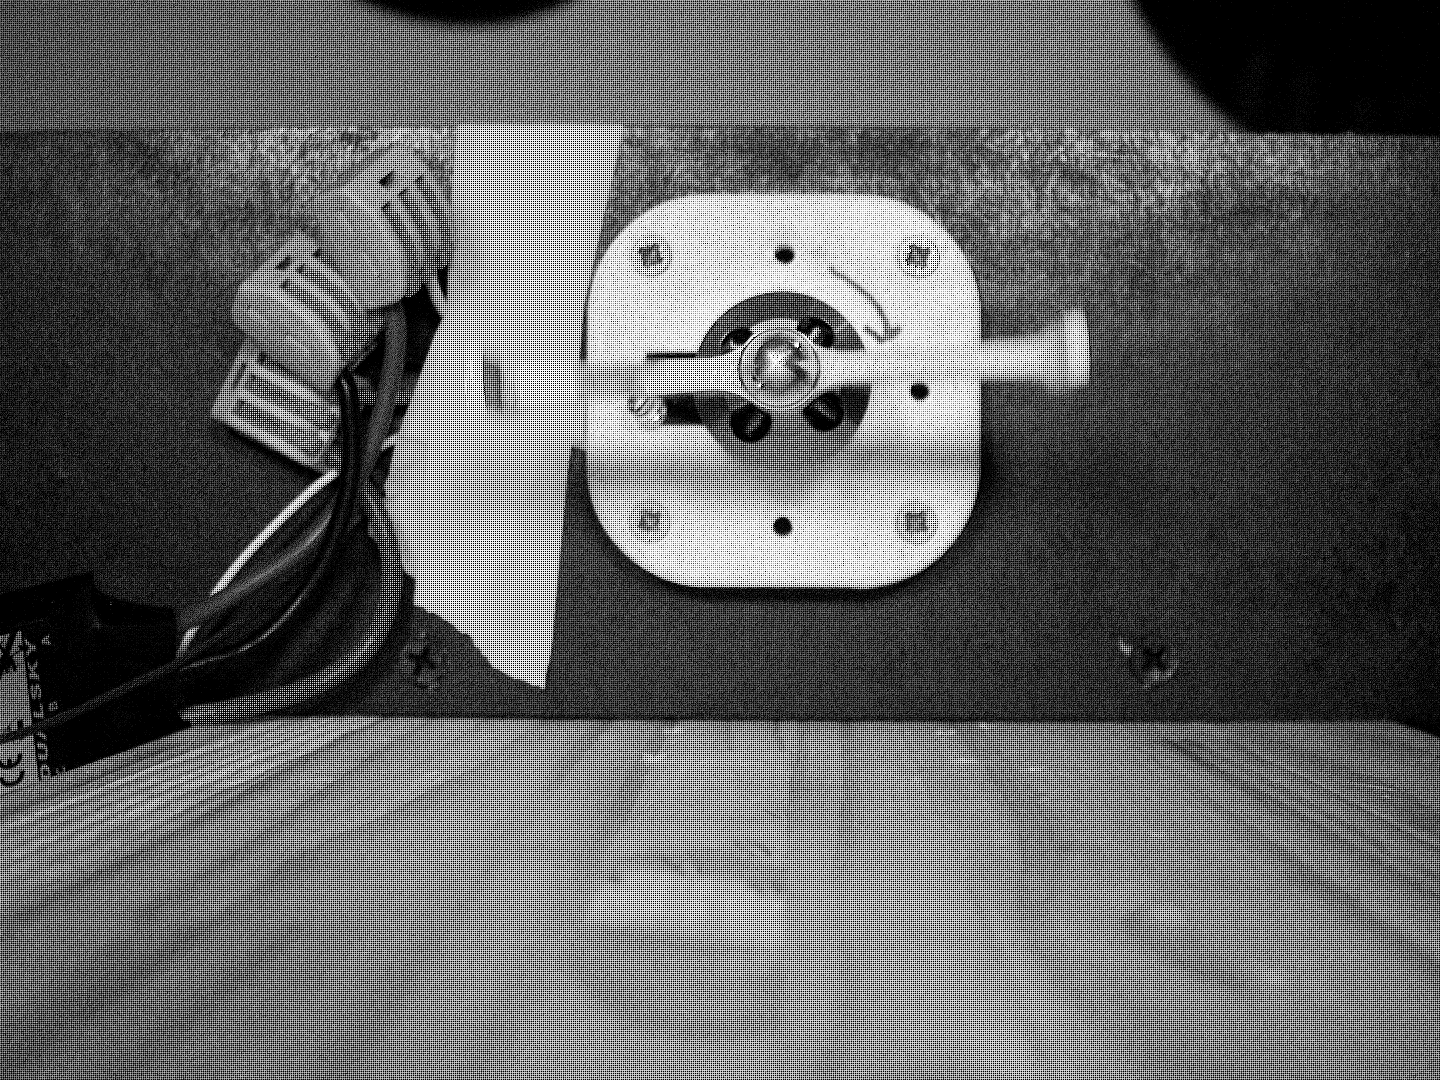
\includegraphics[width=0.8
      \textwidth]{FOTOS_C/8519/0/1.png}
      \caption{Imagen 1 camara 0}
    \end{minipage}
    \begin{minipage}[b]{0.45\textwidth}
      \centering
      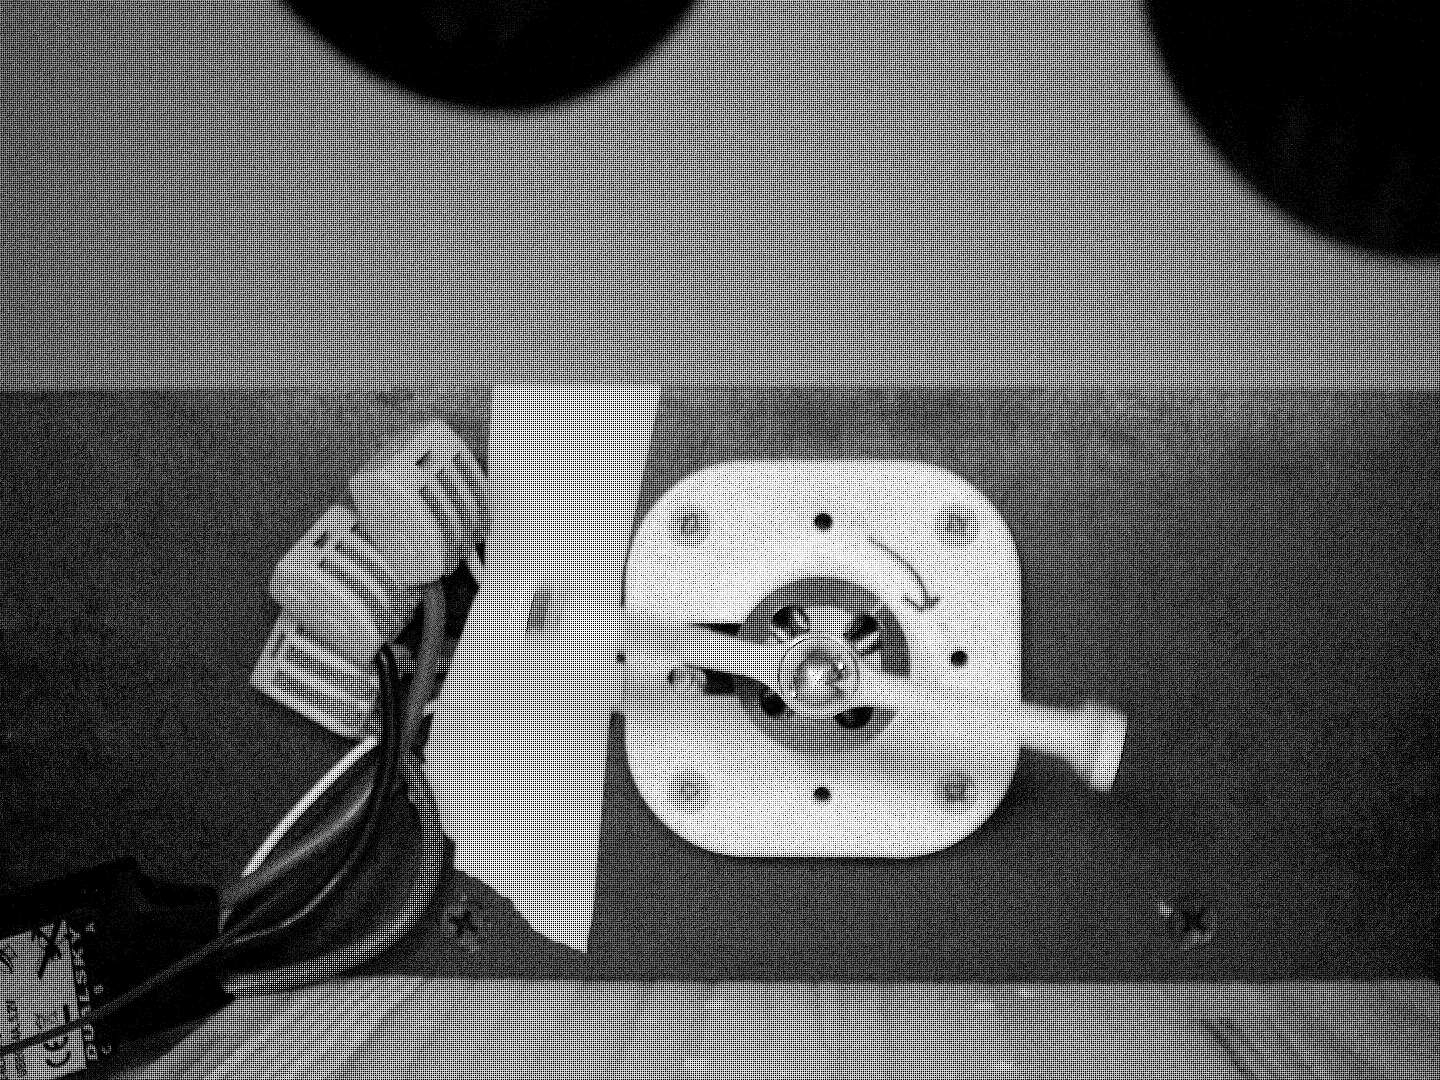
\includegraphics[width=0.8
      \textwidth]{FOTOS_C/8519/1/1.png}
      \caption{Imagen 1 camara 1}
    \end{minipage}
    \begin{minipage}[b]{0.45\textwidth}
      \centering
      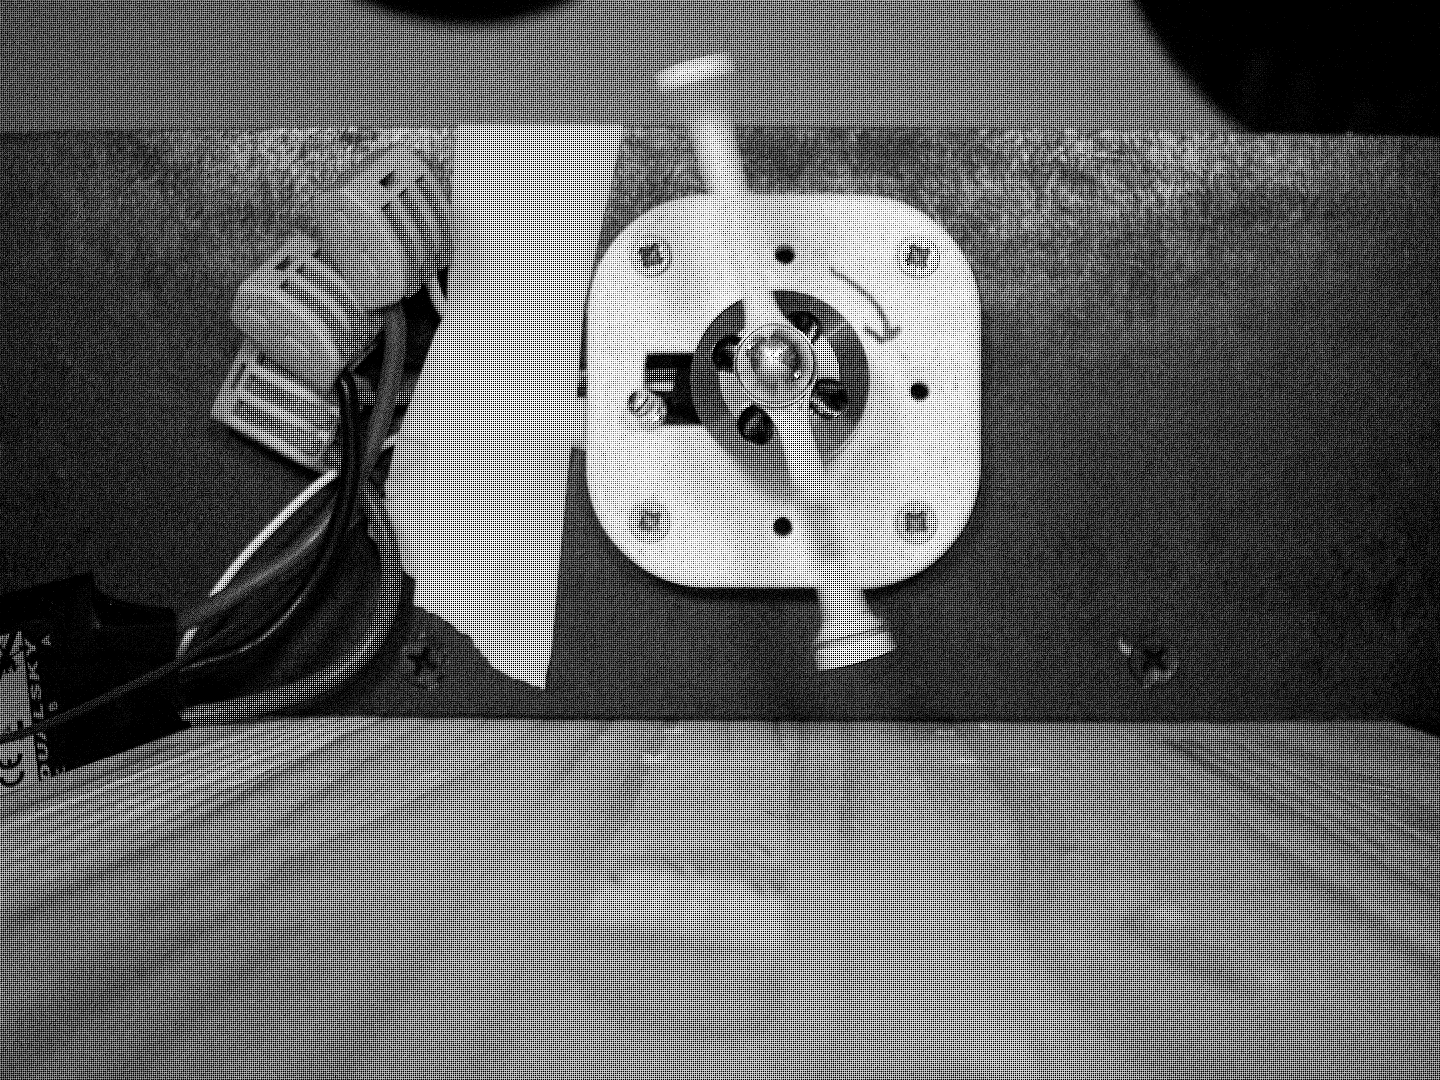
\includegraphics[width=0.8
      \textwidth]{FOTOS_C/8519/0/2.png}
      \caption{Imagen 2 camara 0}
    \end{minipage}
    \begin{minipage}[b]{0.45\textwidth}
      \centering
      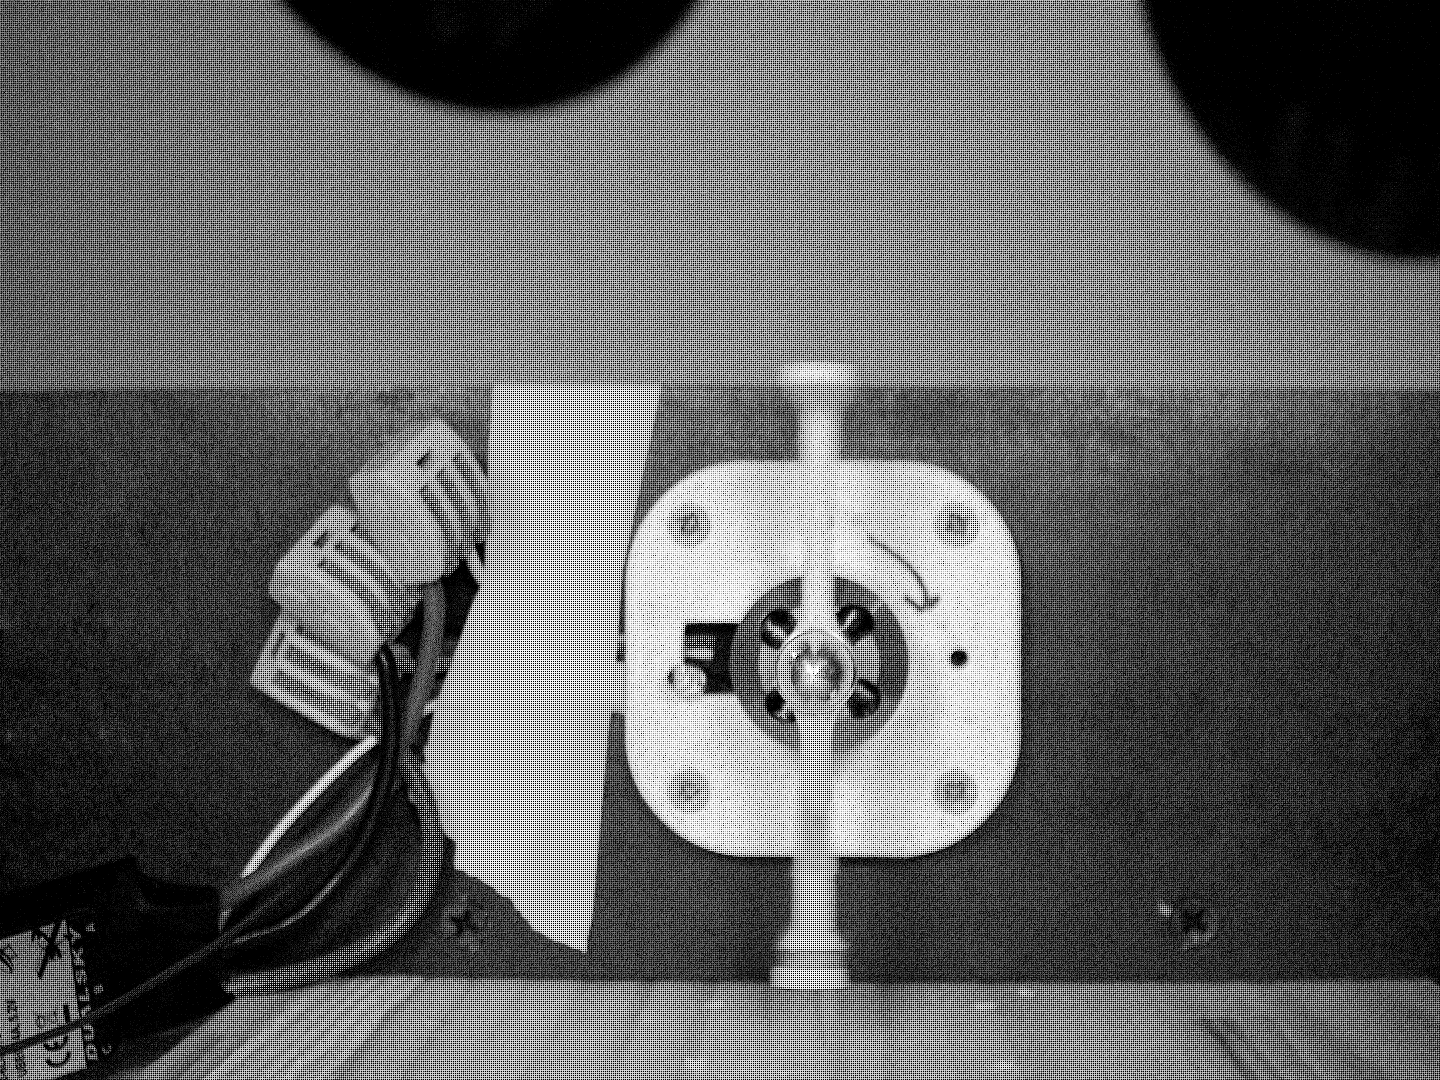
\includegraphics[width=0.8
      \textwidth]{FOTOS_C/8519/1/2.png}
      \caption{Imagen 2 camara 1}
    \end{minipage}
    \begin{minipage}[b]{0.45\textwidth}
      \centering
      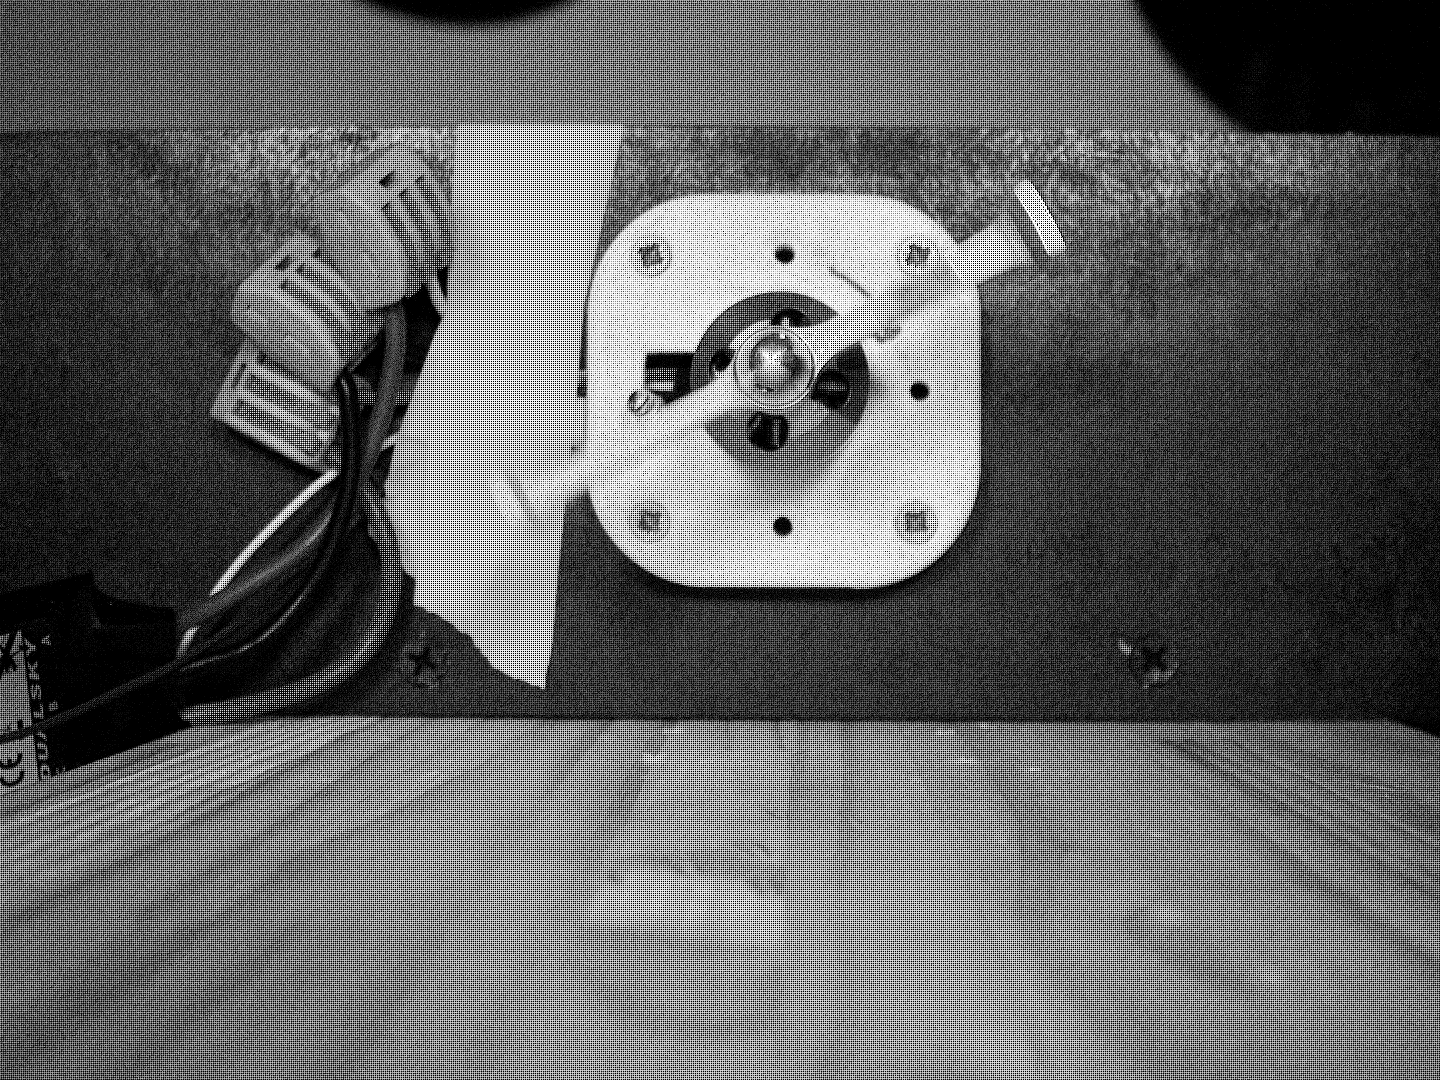
\includegraphics[width=0.8
      \textwidth]{FOTOS_C/8519/0/3.png}
      \caption{Imagen 3 camara 0}
    \end{minipage}
    \begin{minipage}[b]{0.45\textwidth}
      \centering
      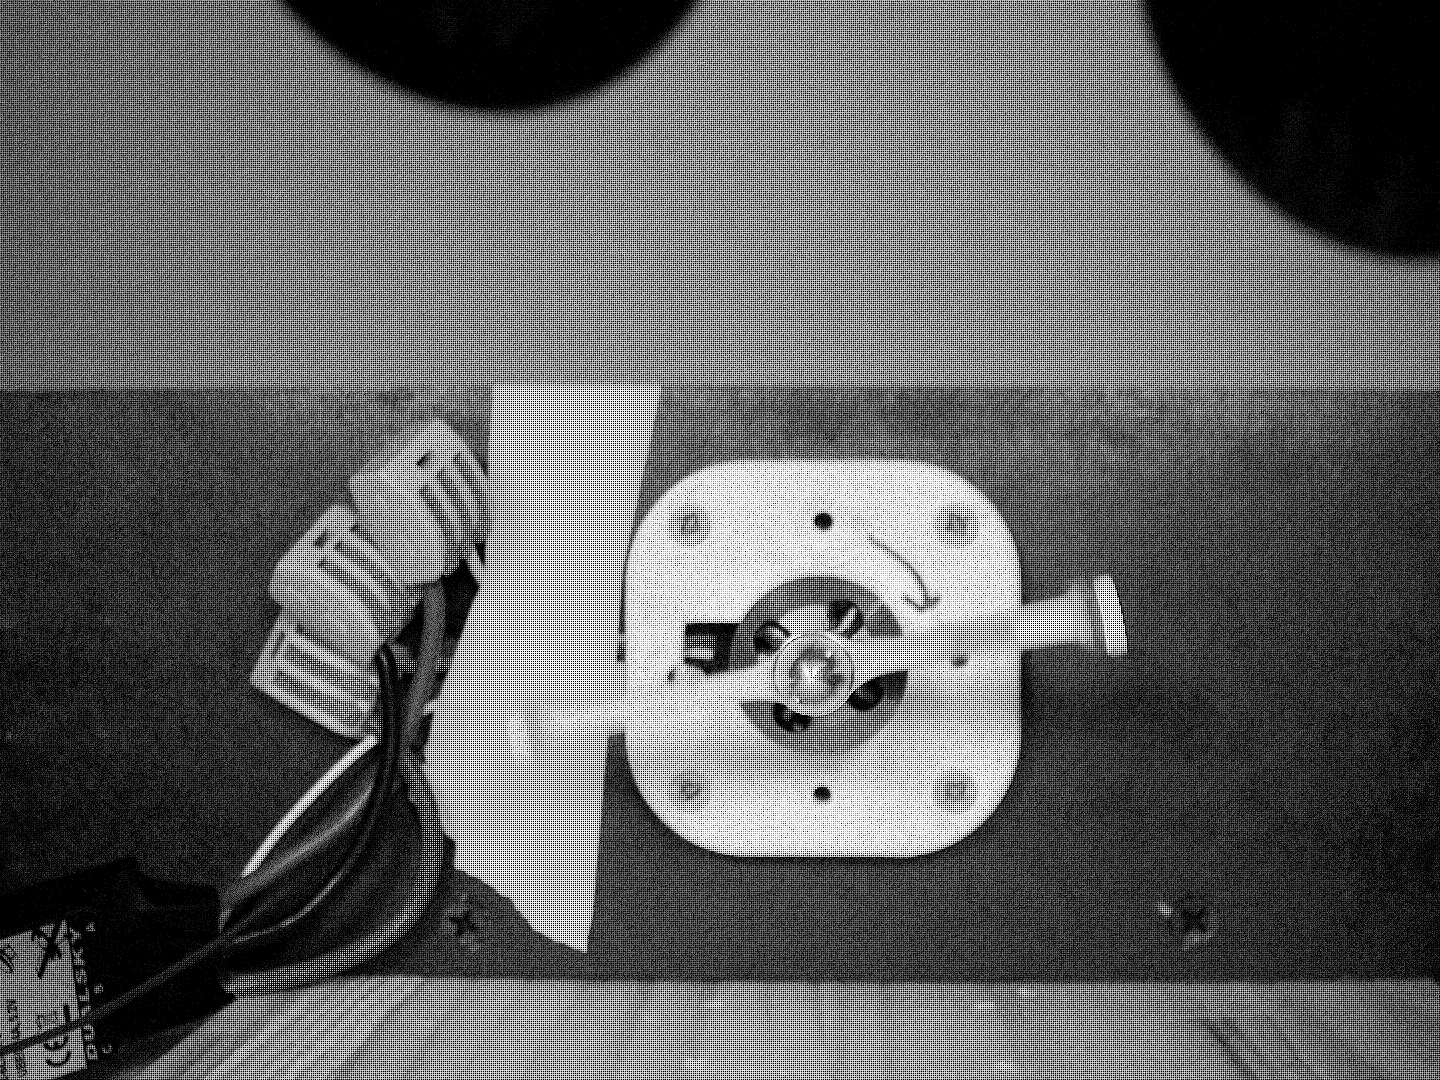
\includegraphics[width=0.8
      \textwidth]{FOTOS_C/8519/1/3.png}
      \caption{Imagen 3 camara 1}
    \end{minipage}
    \begin{minipage}[b]{0.45\textwidth}
      \centering
      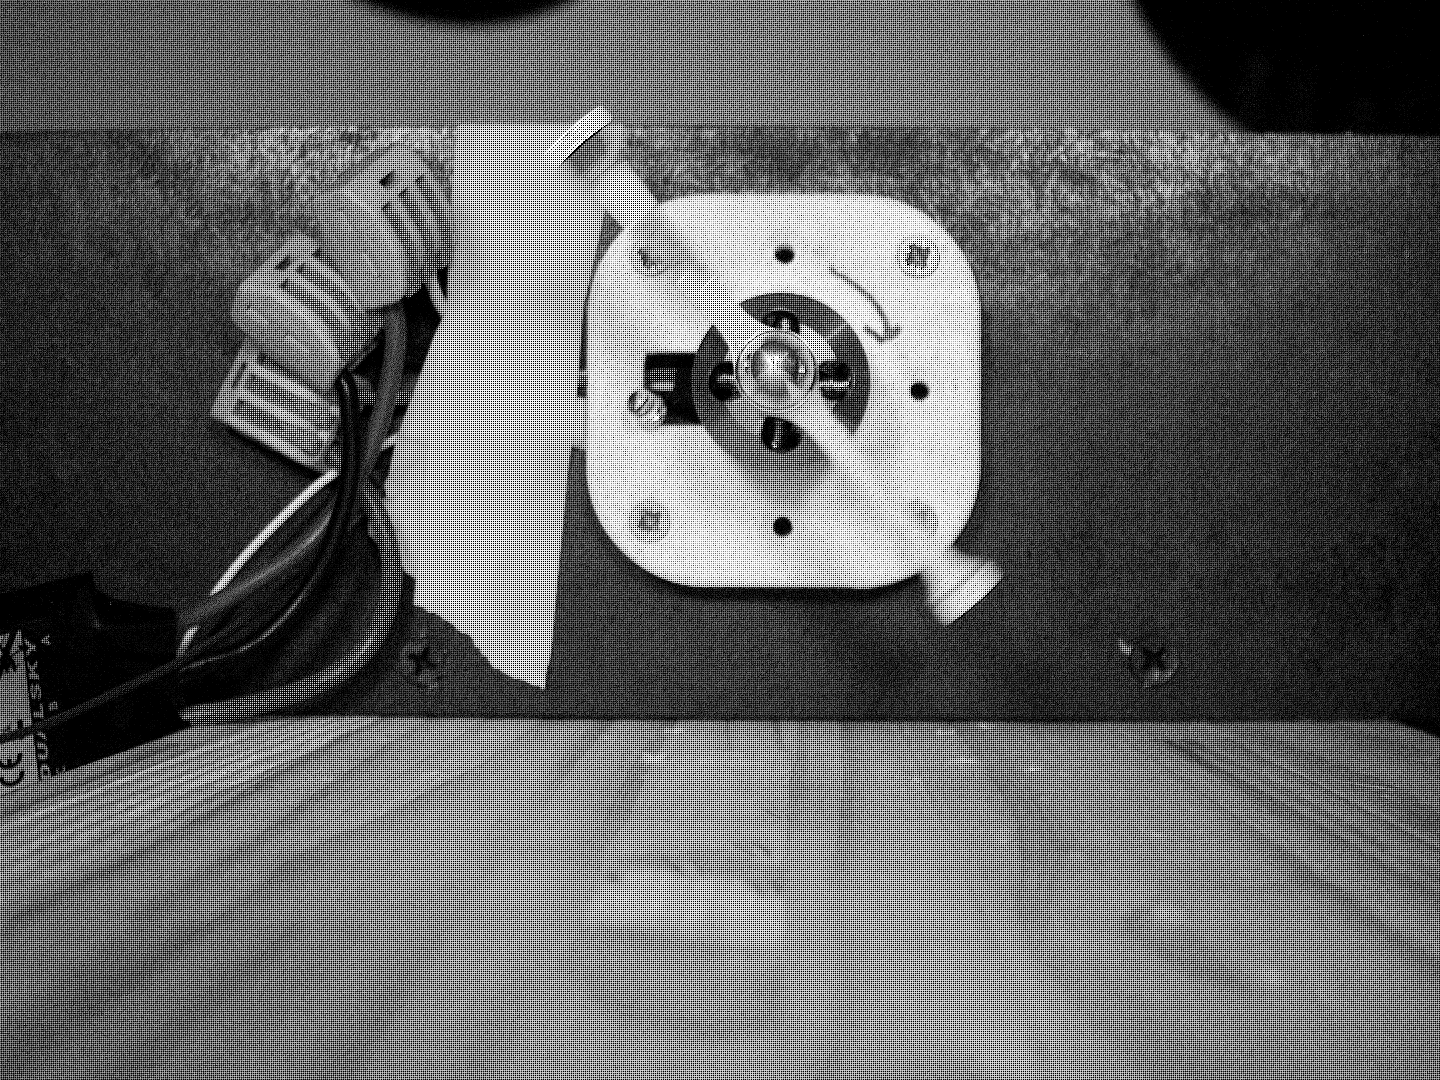
\includegraphics[width=0.8
      \textwidth]{FOTOS_C/8519/0/4.png}
      \caption{Imagen 4 camara 0}
    \end{minipage}
    \begin{minipage}[b]{0.45\textwidth}
      \centering
      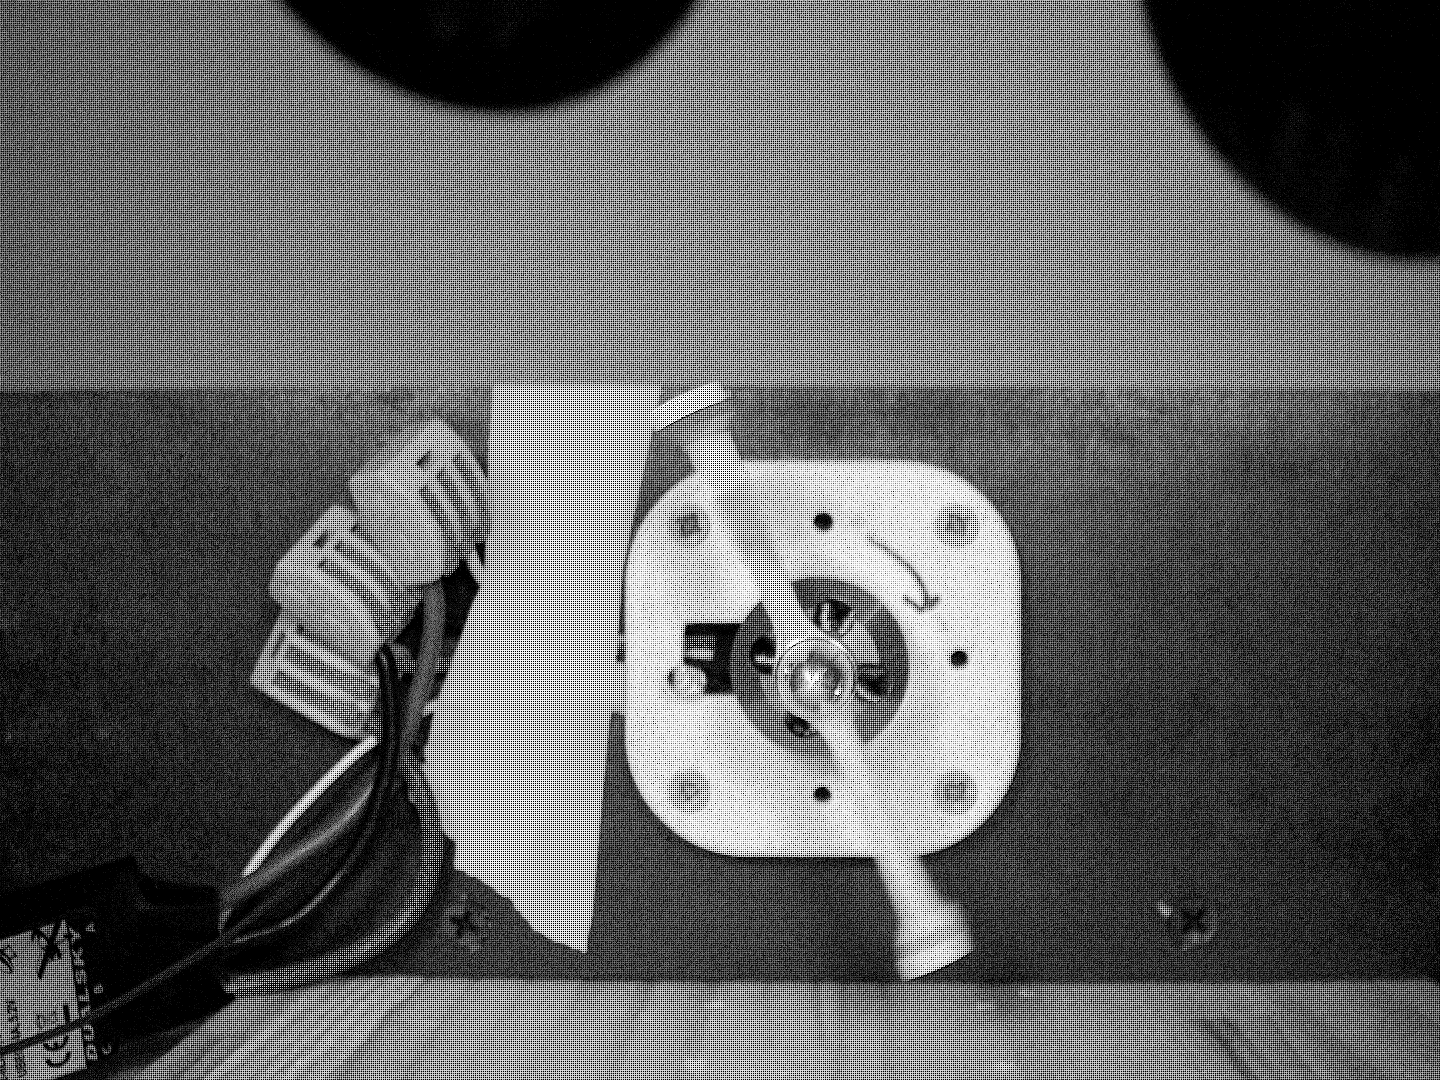
\includegraphics[width=0.8
      \textwidth]{FOTOS_C/8519/1/4.png}
      \caption{Imagen 4 camara 1}
    \end{minipage}
\end{figure}

\newpage
\noindent A continuación se mostrarán las fotos de una medición a 12055 RPM.

\begin{figure}[H]
    \centering
    \begin{minipage}[b]{0.45\textwidth}
      \centering
      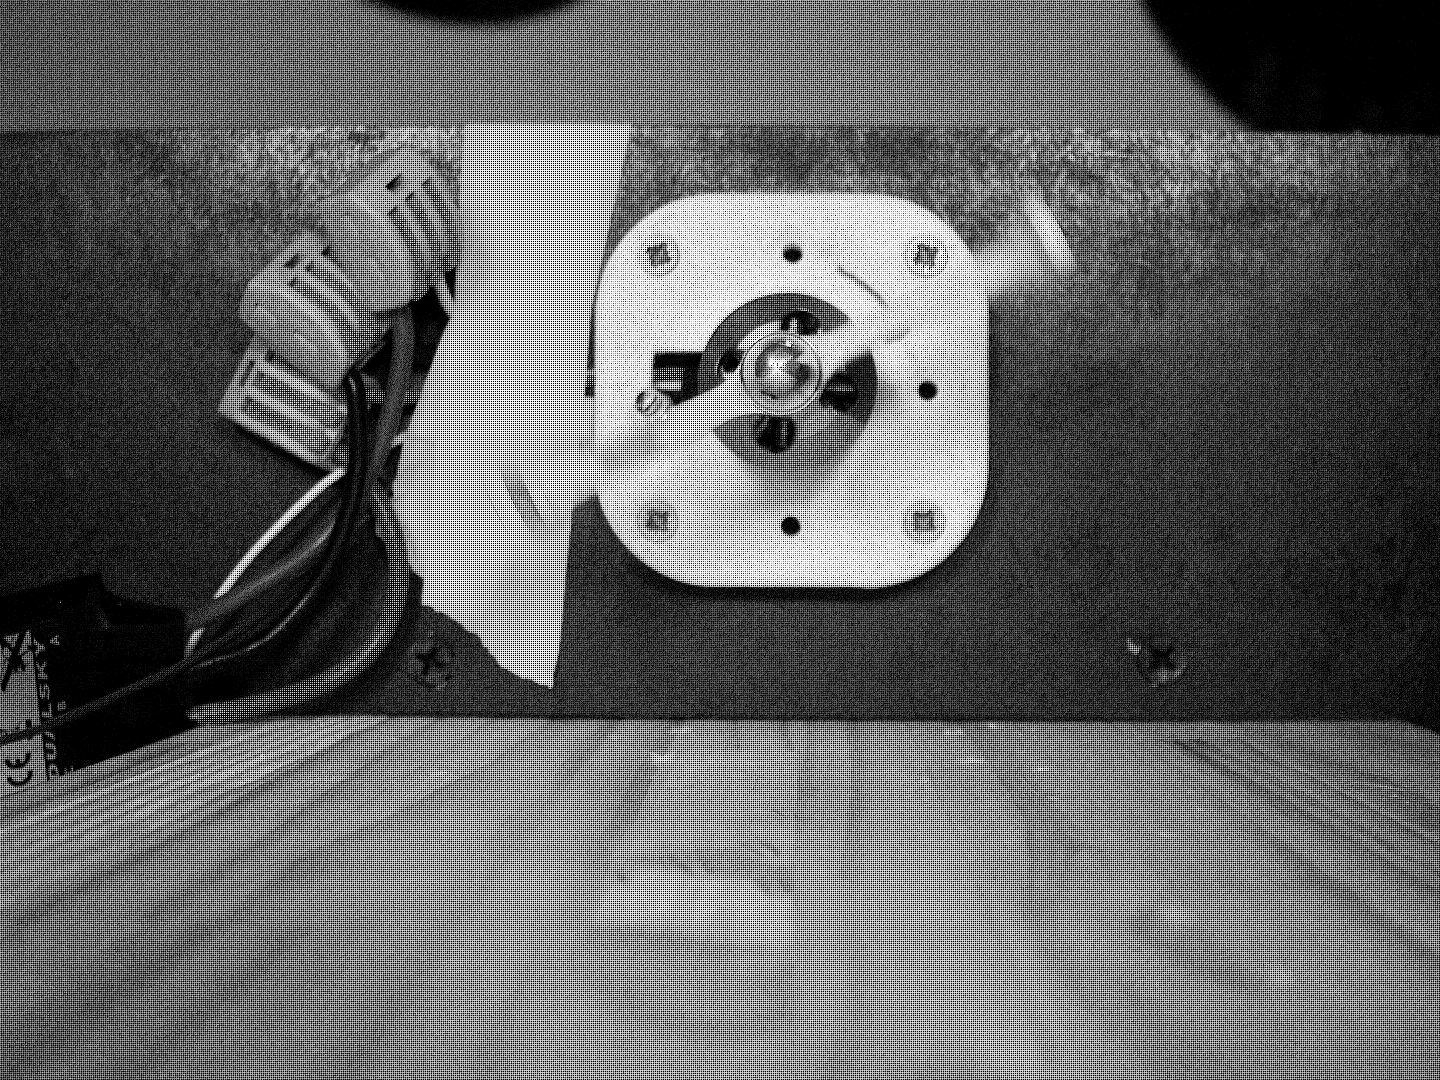
\includegraphics[width=0.8
      \textwidth]{FOTOS_C/12055/0/1.png}
      \caption{Imagen 1 camara 0}
    \end{minipage}
    \begin{minipage}[b]{0.45\textwidth}
      \centering
      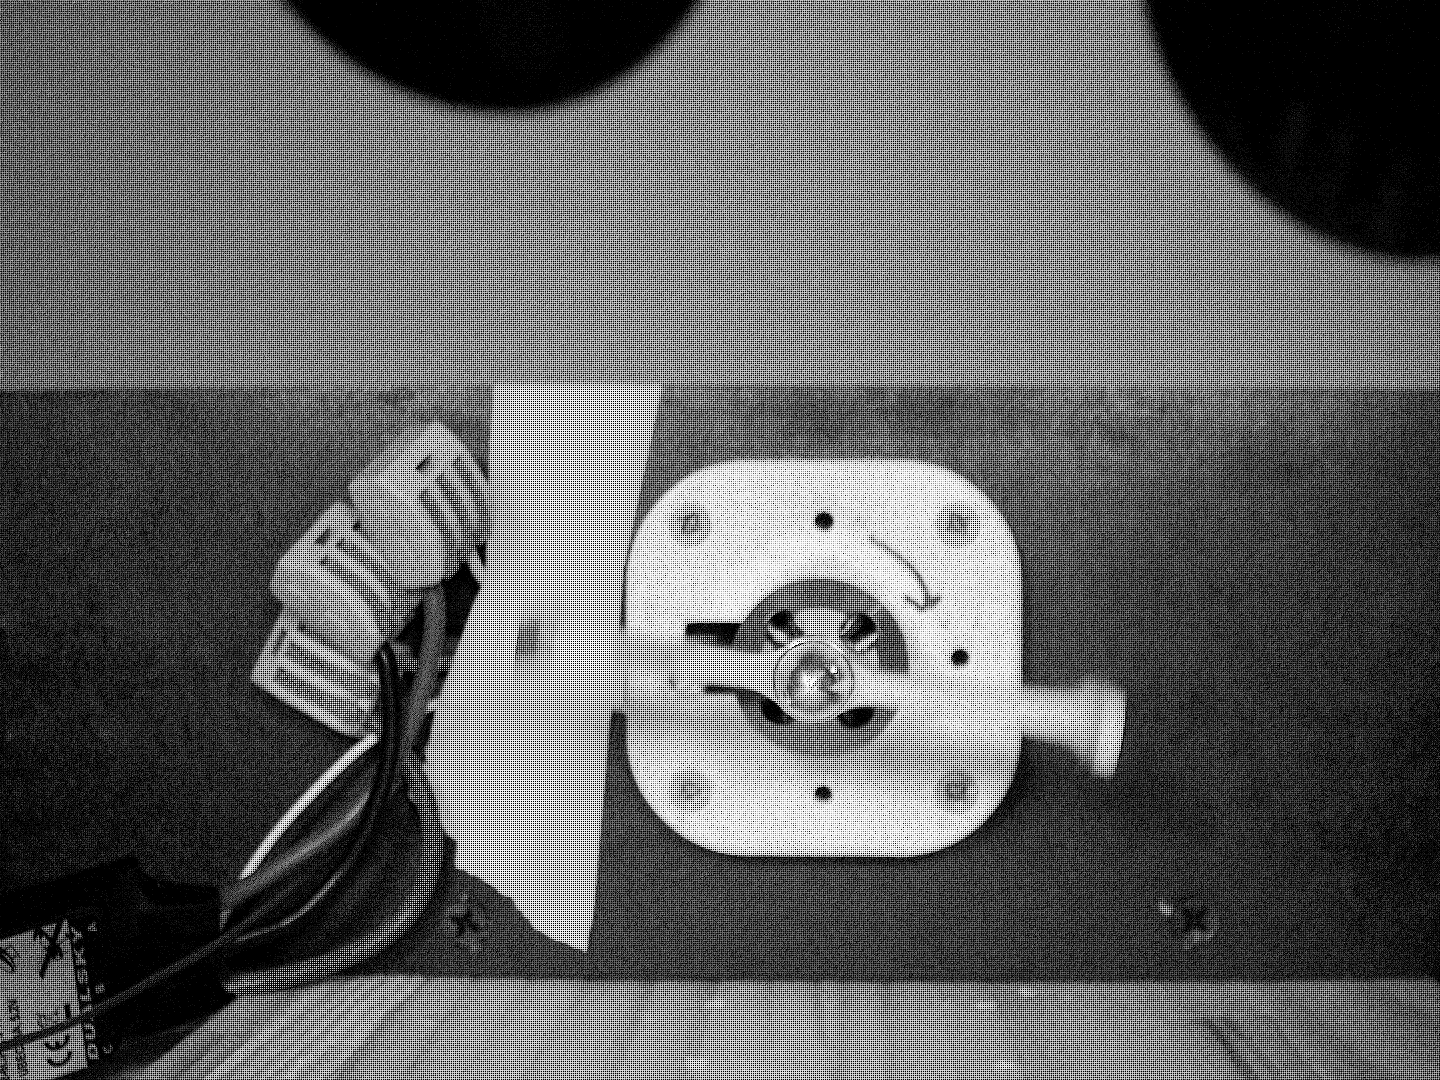
\includegraphics[width=0.8
      \textwidth]{FOTOS_C/12055/1/1.png}
      \caption{Imagen 1 camara 1}
    \end{minipage}
    \begin{minipage}[b]{0.45\textwidth}
      \centering
      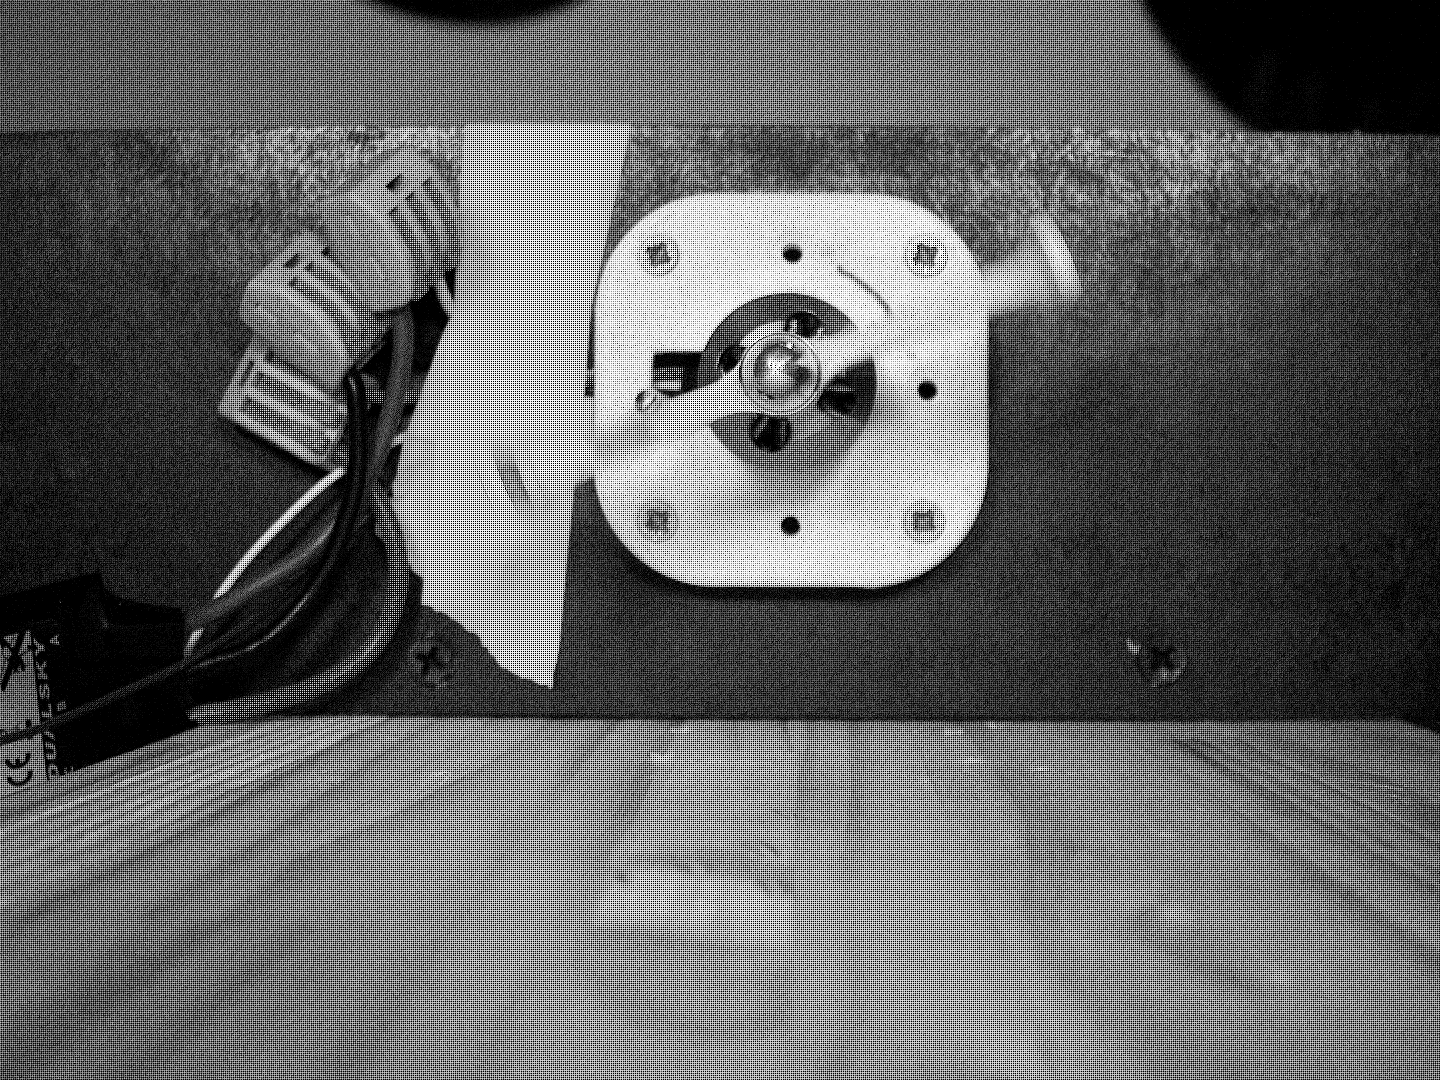
\includegraphics[width=0.8
      \textwidth]{FOTOS_C/12055/0/2.png}
      \caption{Imagen 2 camara 0}
    \end{minipage}
    \begin{minipage}[b]{0.45\textwidth}
      \centering
      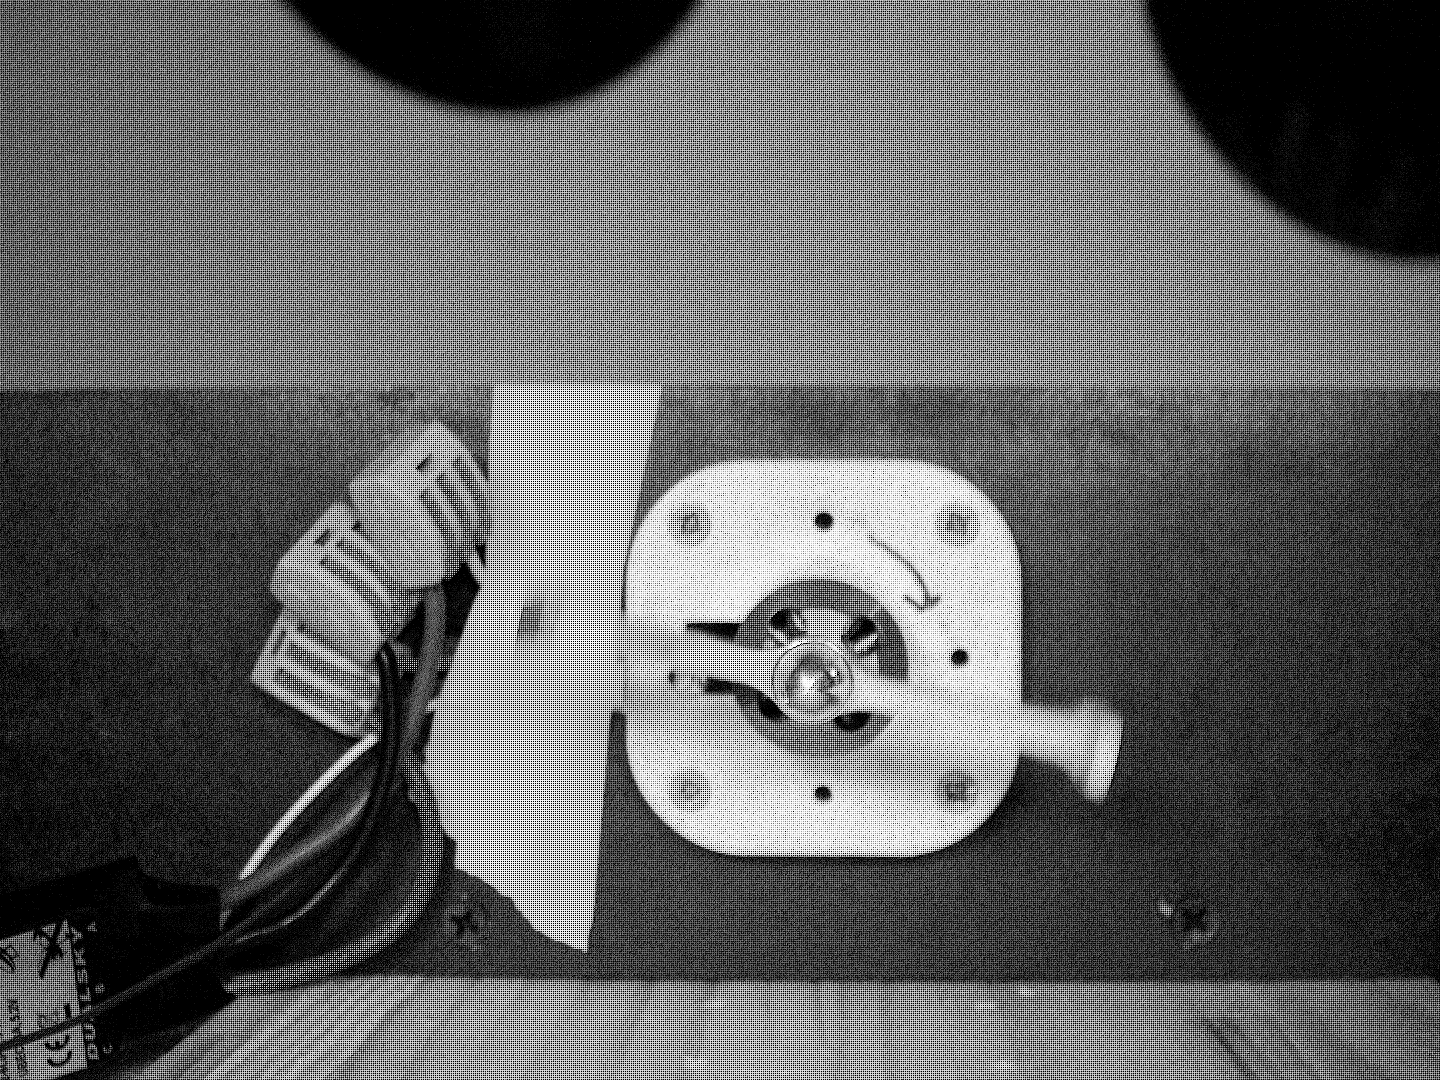
\includegraphics[width=0.8
      \textwidth]{FOTOS_C/12055/1/2.png}
      \caption{Imagen 2 camara 1}
    \end{minipage}
    \begin{minipage}[b]{0.45\textwidth}
      \centering
      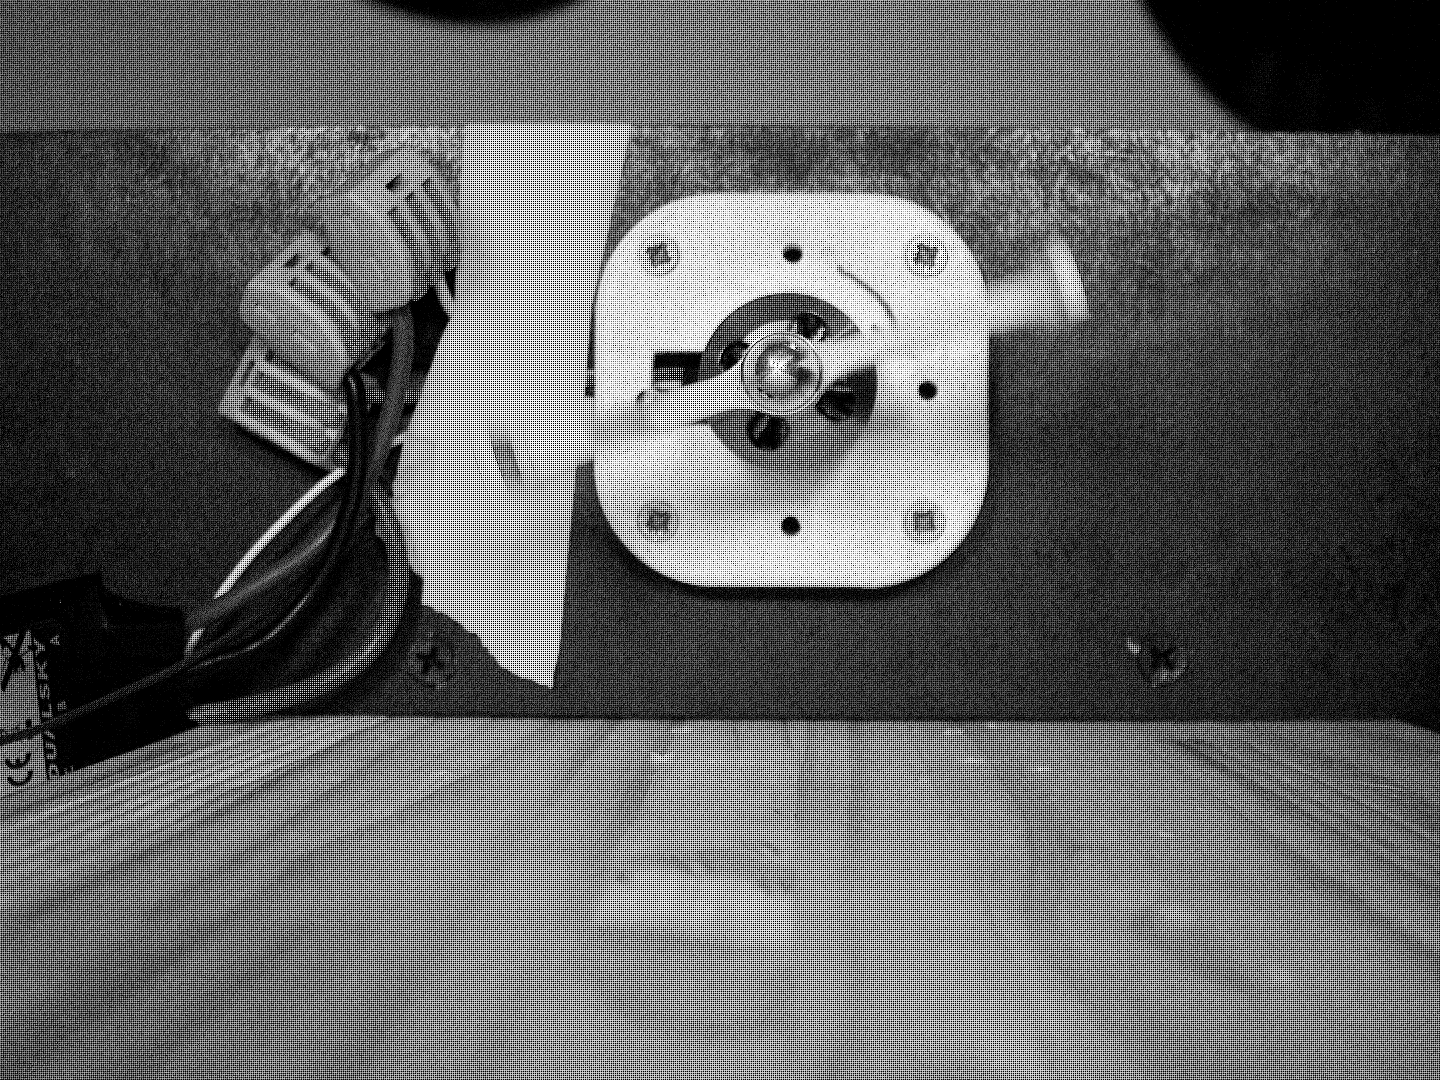
\includegraphics[width=0.8
      \textwidth]{FOTOS_C/12055/0/3.png}
      \caption{Imagen 3 camara 0}
    \end{minipage}
    \begin{minipage}[b]{0.45\textwidth}
      \centering
      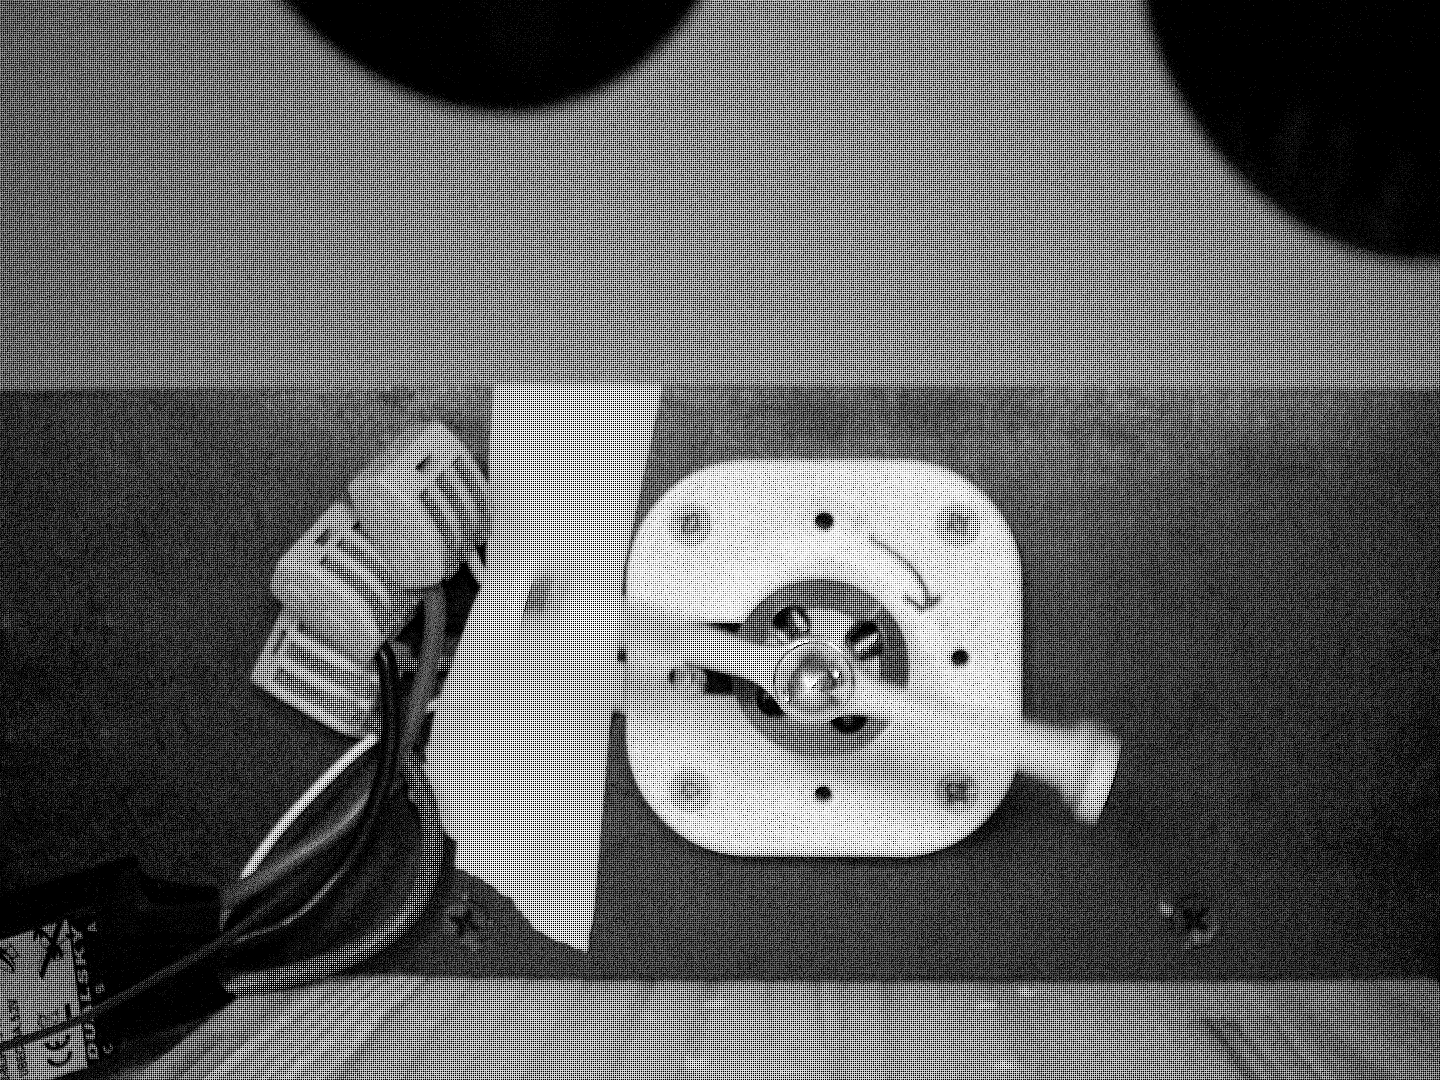
\includegraphics[width=0.8
      \textwidth]{FOTOS_C/12055/1/3.png}
      \caption{Imagen 3 camara 1}
    \end{minipage}
    \begin{minipage}[b]{0.45\textwidth}
      \centering
      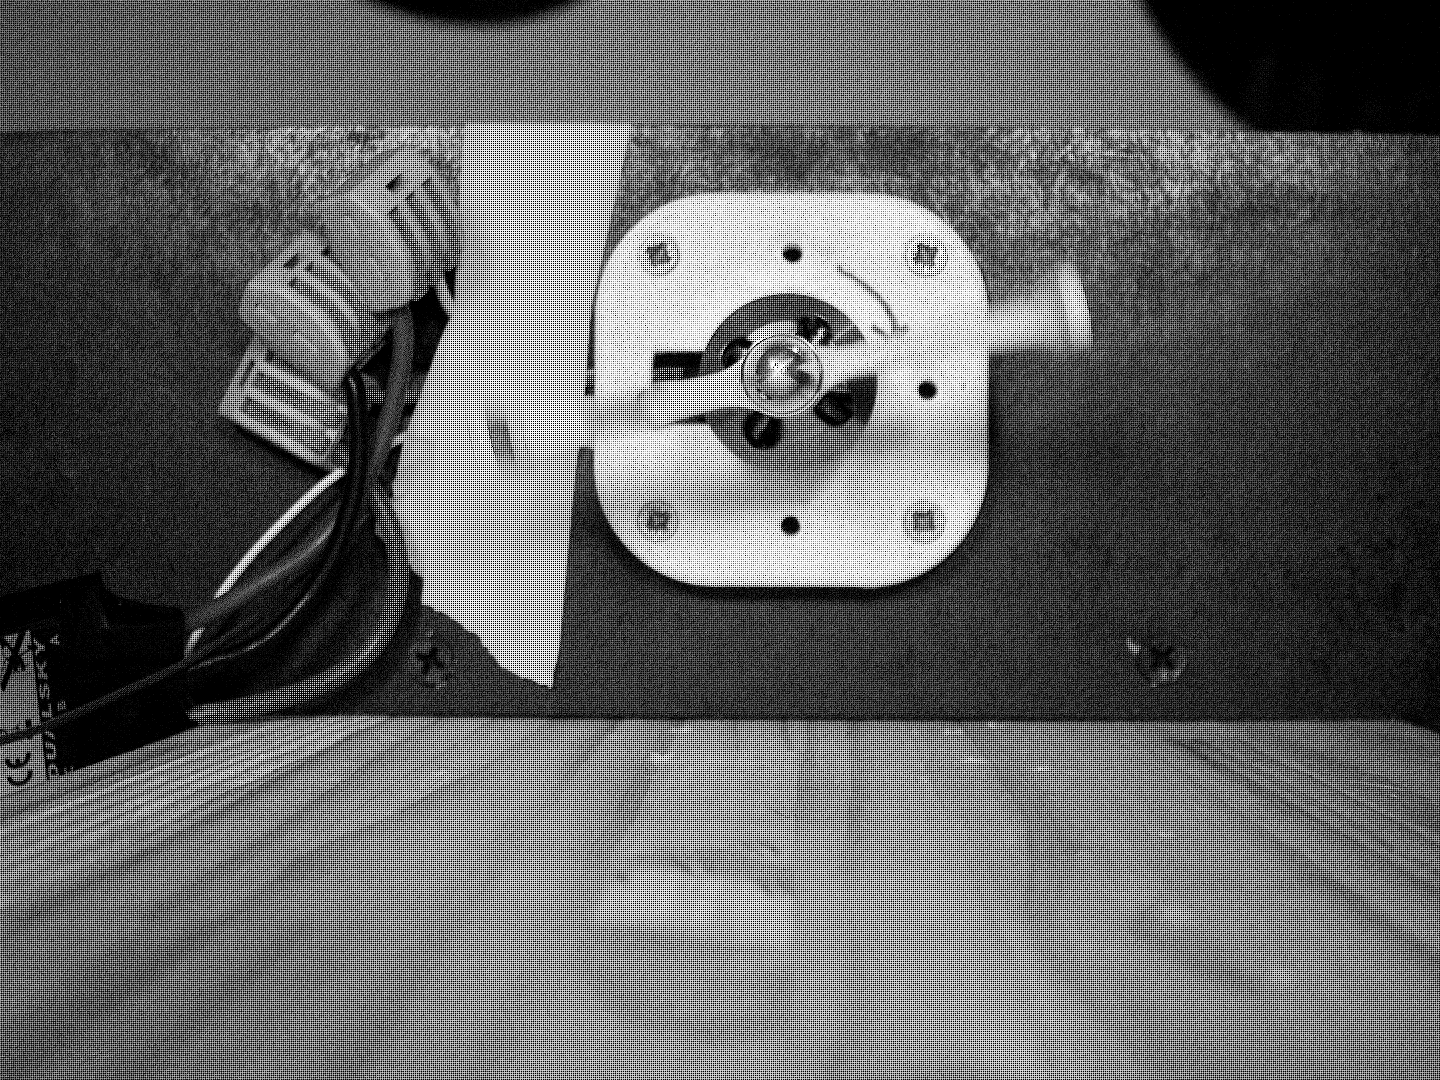
\includegraphics[width=0.8
      \textwidth]{FOTOS_C/12055/0/4.png}
      \caption{Imagen 4 camara 0}
    \end{minipage}
    \begin{minipage}[b]{0.45\textwidth}
      \centering
      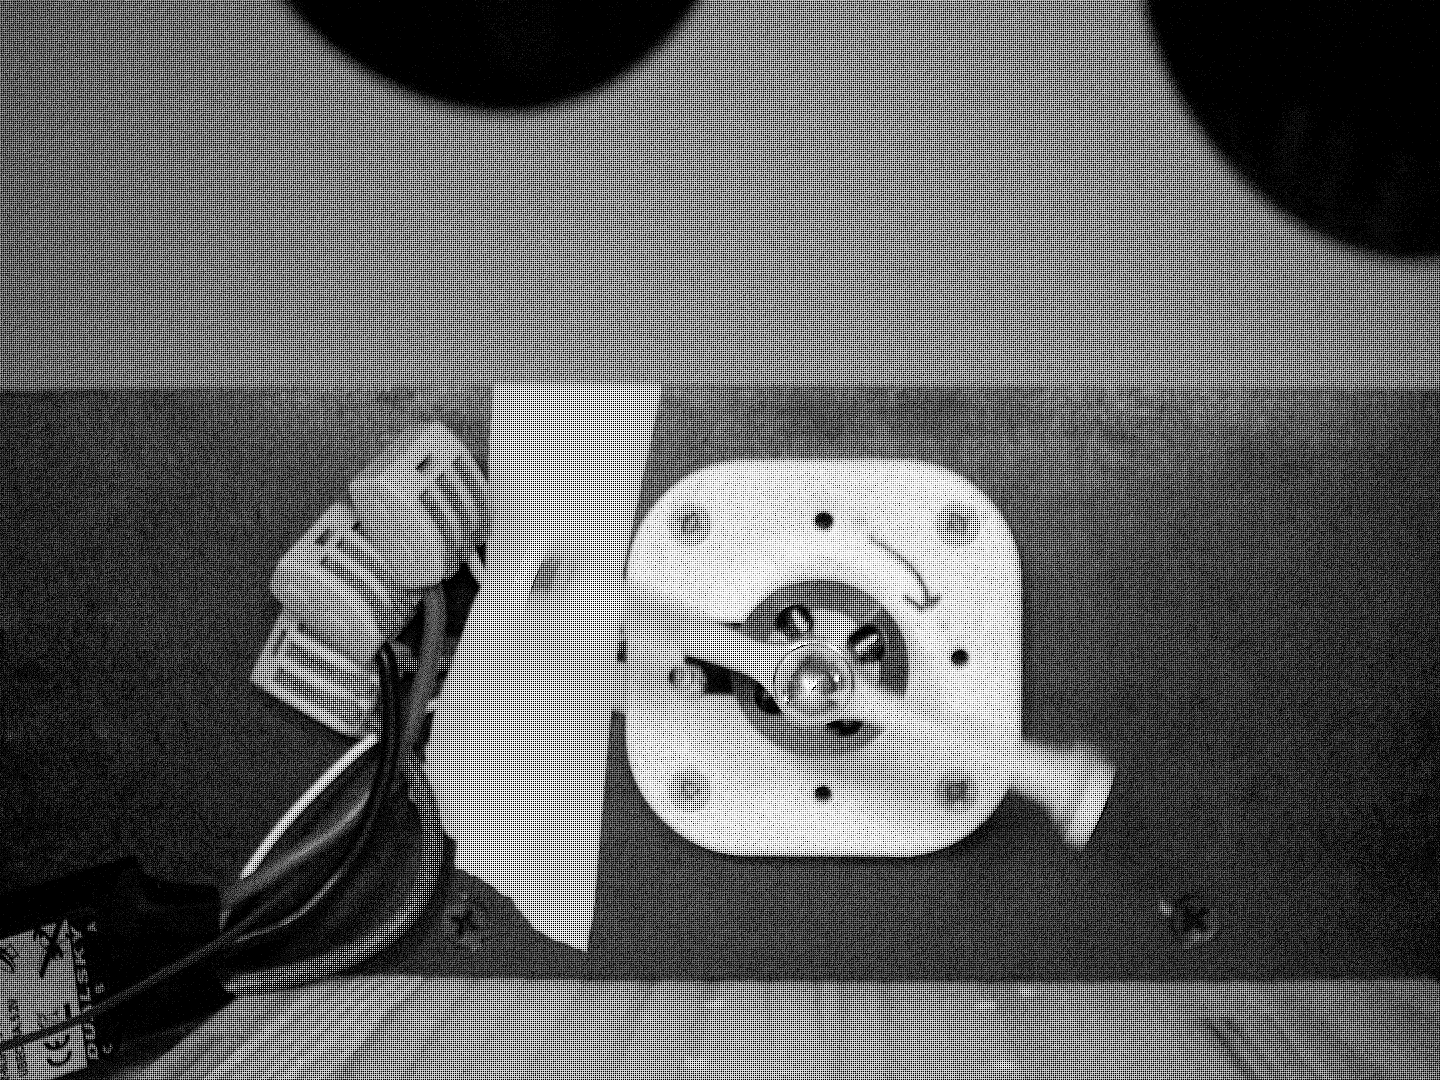
\includegraphics[width=0.8
      \textwidth]{FOTOS_C/12055/1/4.png}
      \caption{Imagen 4 camara 1}
    \end{minipage}
\end{figure}

\noindent De esta última toma, es interesante notar que todas las fotos son prácticamente iguales en posición. Esto se debe a que la hélice giraba a aproximadamente la misma frecuencia que los FPS.

\newpage
Además, se realizó una medición a 1 FPS para verificar los resultados.

\begin{figure}[H]
  \centering
  \begin{minipage}[b]{0.45\textwidth}
    \centering
    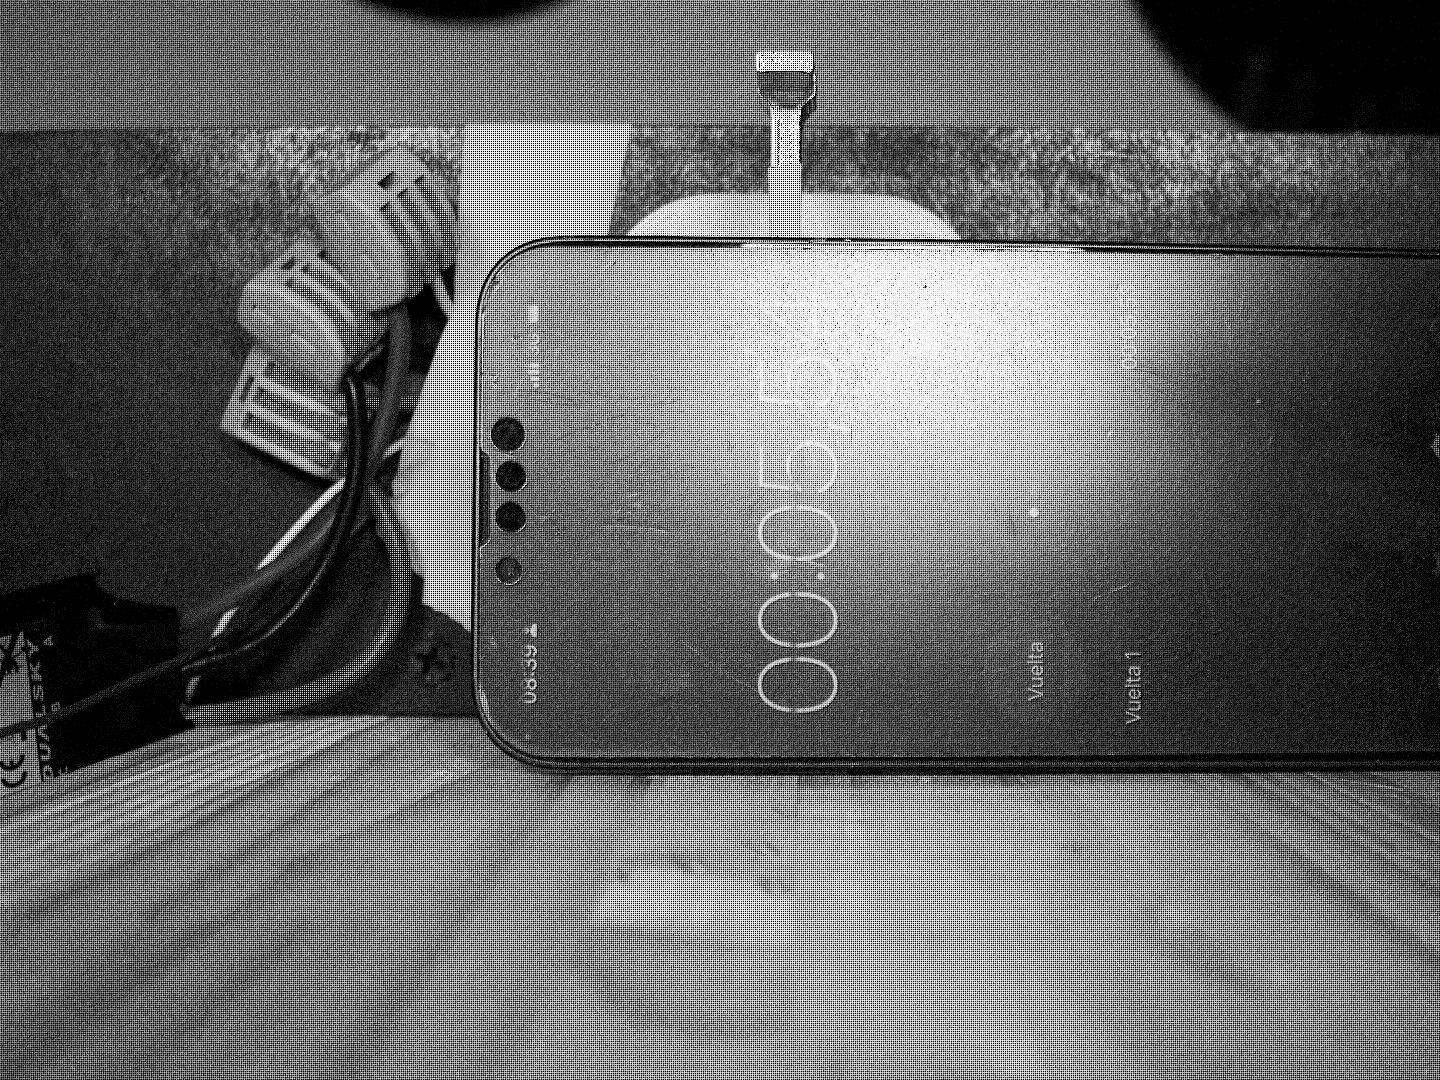
\includegraphics[width=0.8
    \textwidth]{FOTOS_C/1/0/1.png}
    \caption{Imagen 1 camara 0}
  \end{minipage}
  \begin{minipage}[b]{0.45\textwidth}
    \centering
    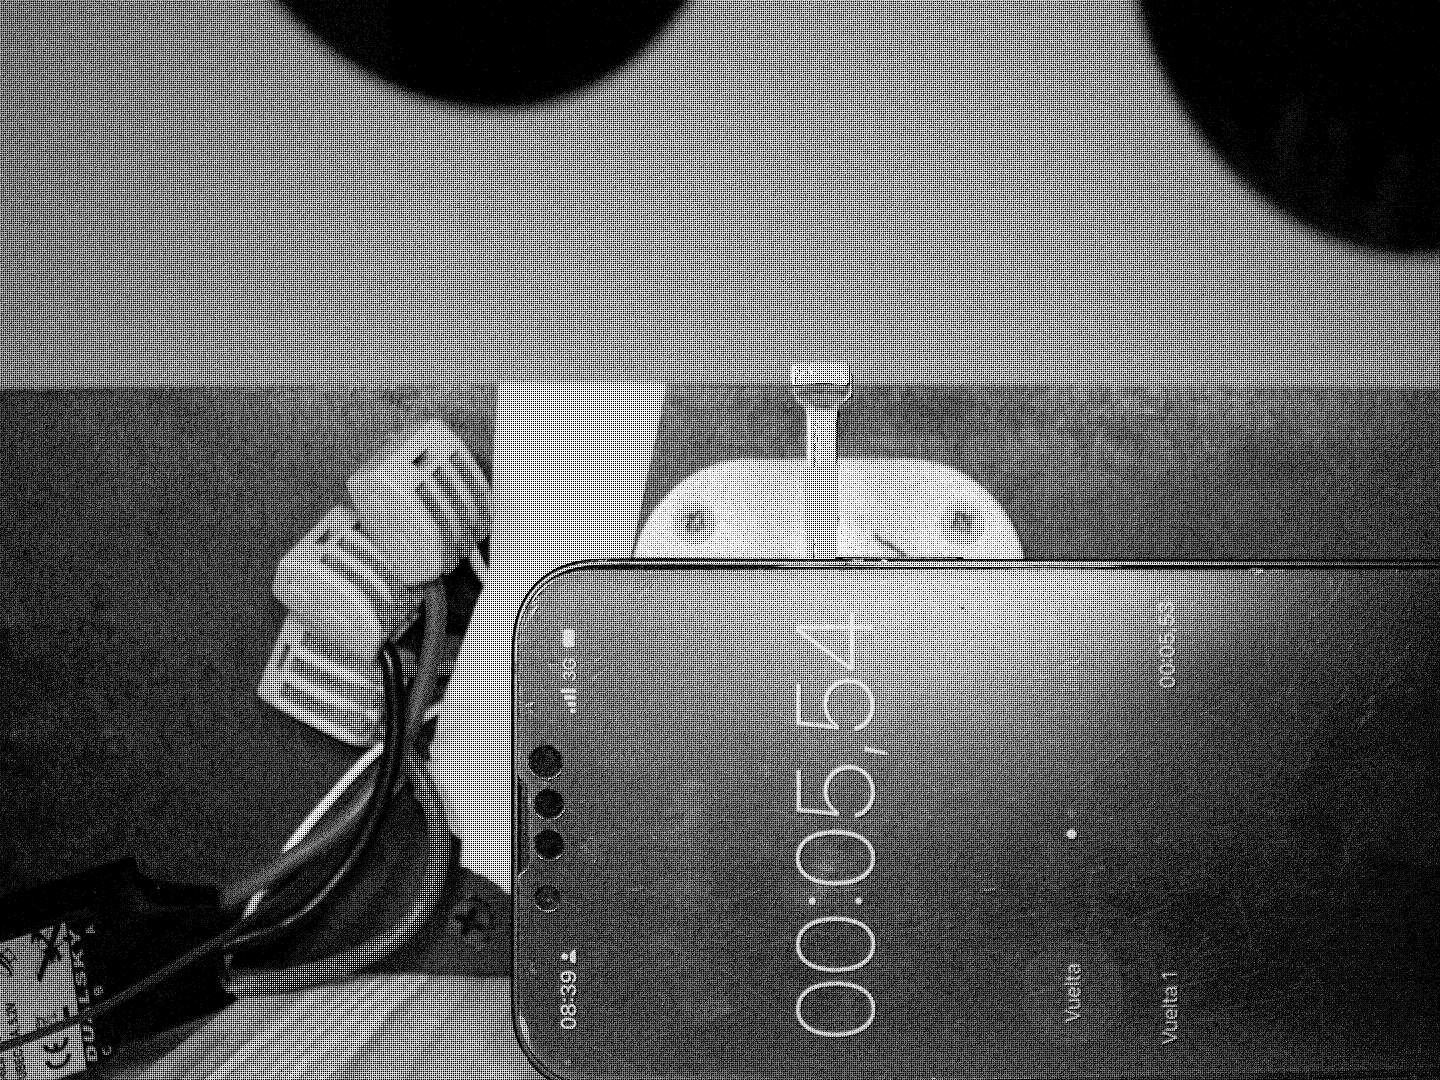
\includegraphics[width=0.8
    \textwidth]{FOTOS_C/1/1/1.png}
    \caption{Imagen 1 camara 1}
  \end{minipage}
  \begin{minipage}[b]{0.45\textwidth}
    \centering
    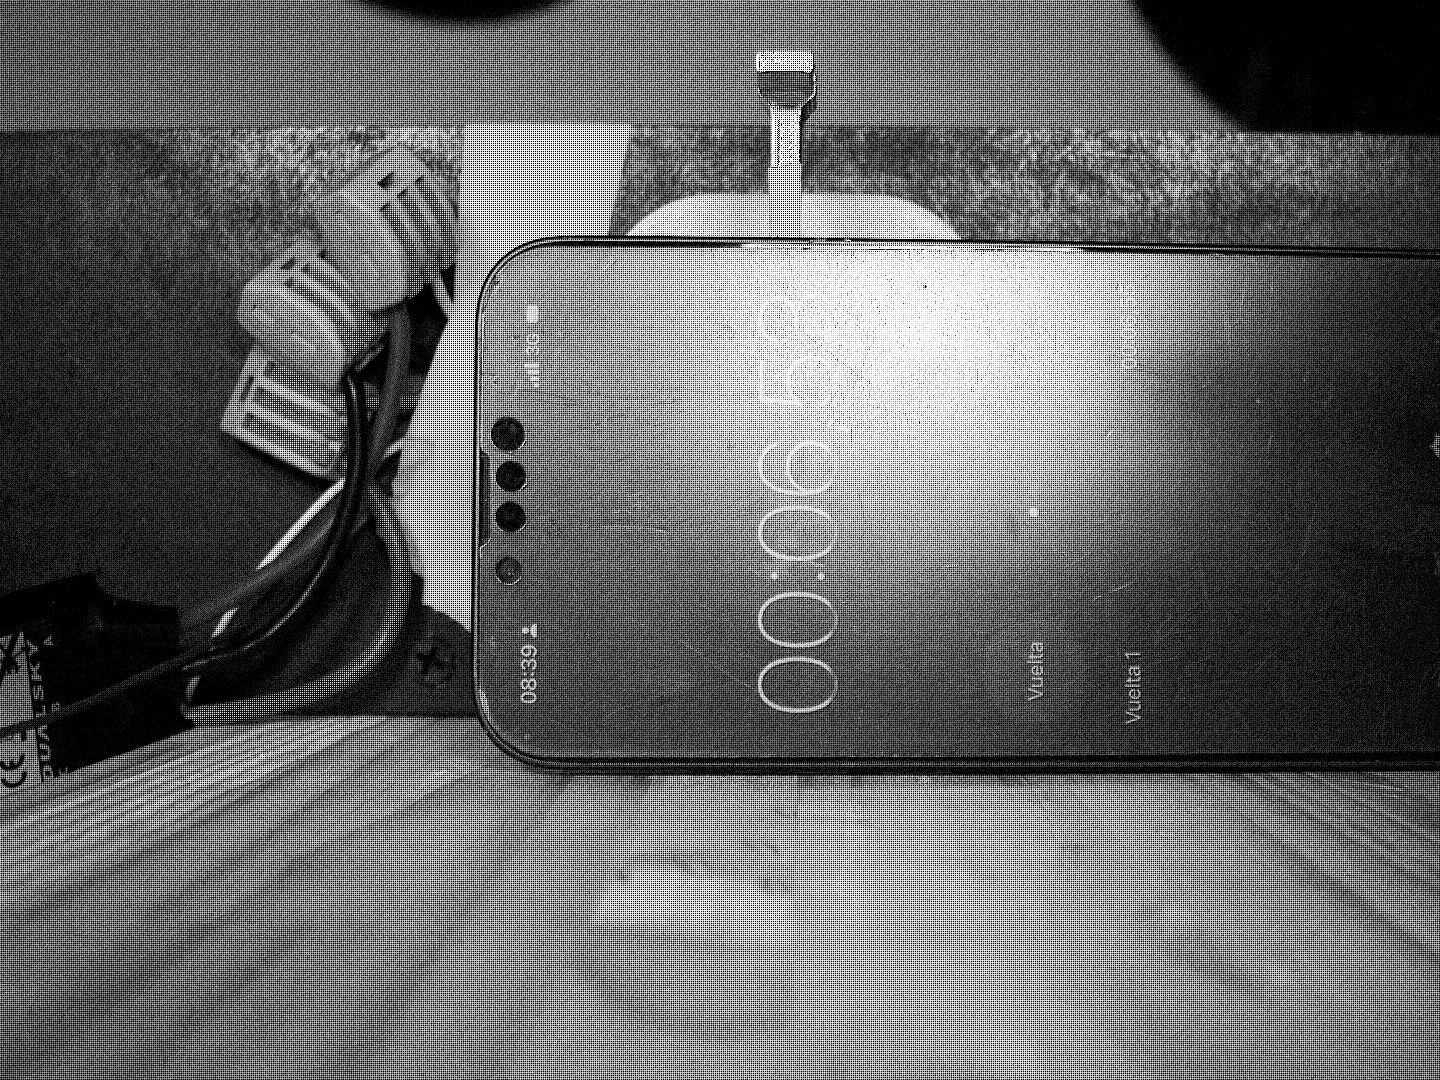
\includegraphics[width=0.8
    \textwidth]{FOTOS_C/1/0/2.png}
    \caption{Imagen 2 camara 0}
  \end{minipage}
  \begin{minipage}[b]{0.45\textwidth}
    \centering
    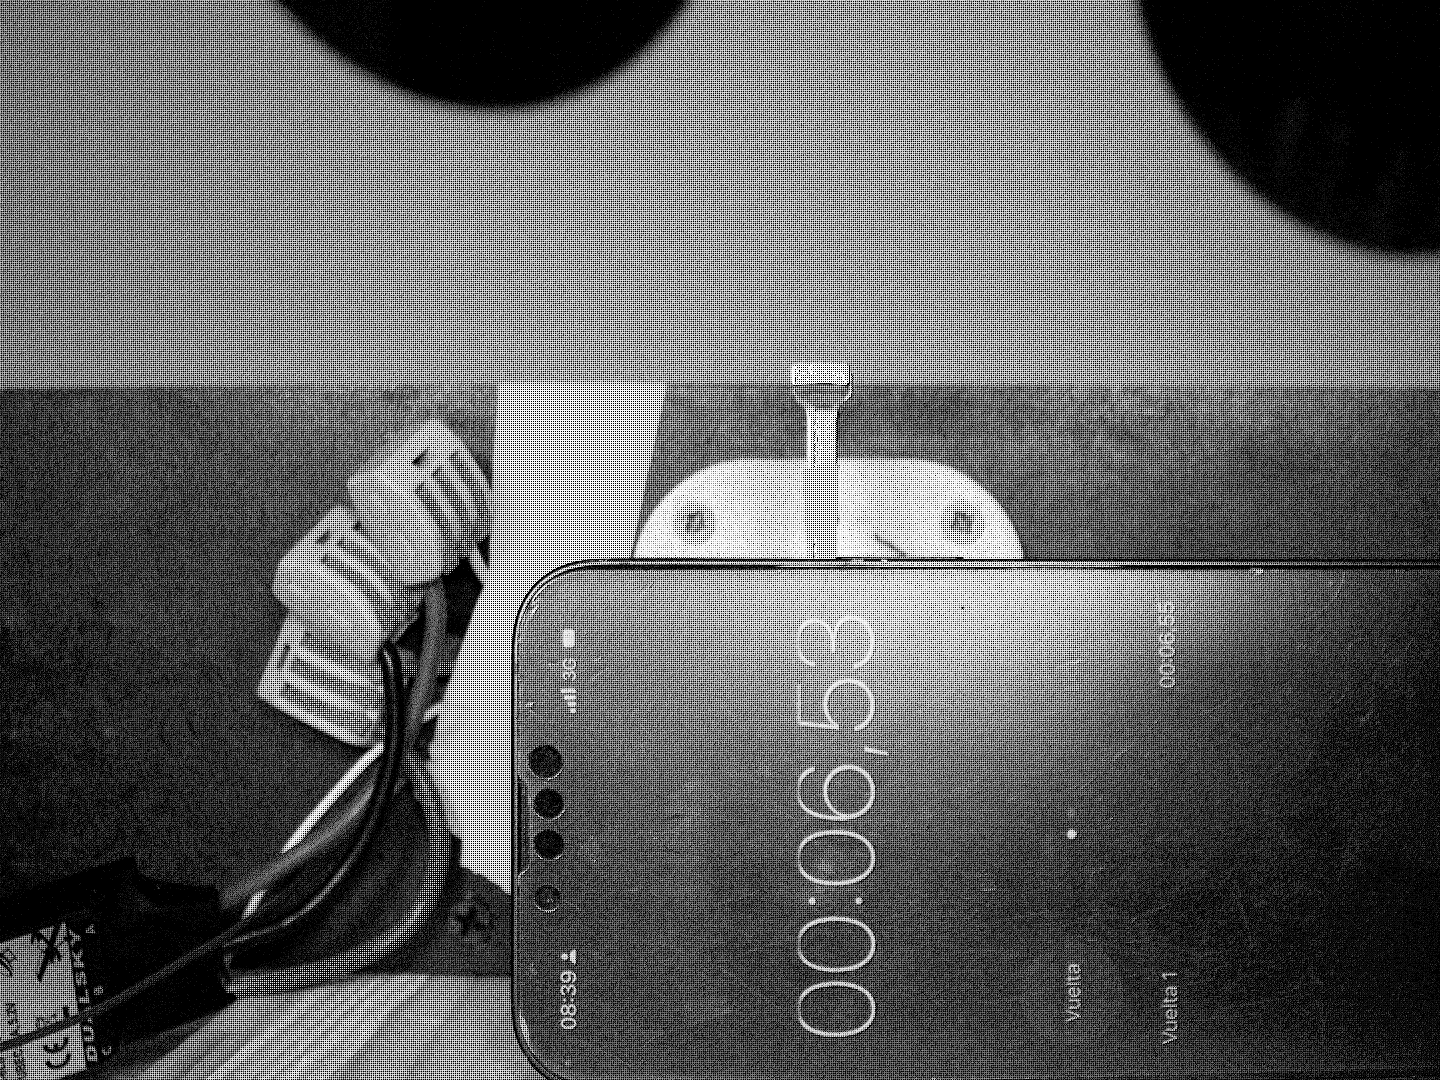
\includegraphics[width=0.8
    \textwidth]{FOTOS_C/1/1/2.png}
    \caption{Imagen 2 camara 1}
  \end{minipage}
  \begin{minipage}[b]{0.45\textwidth}
    \centering
    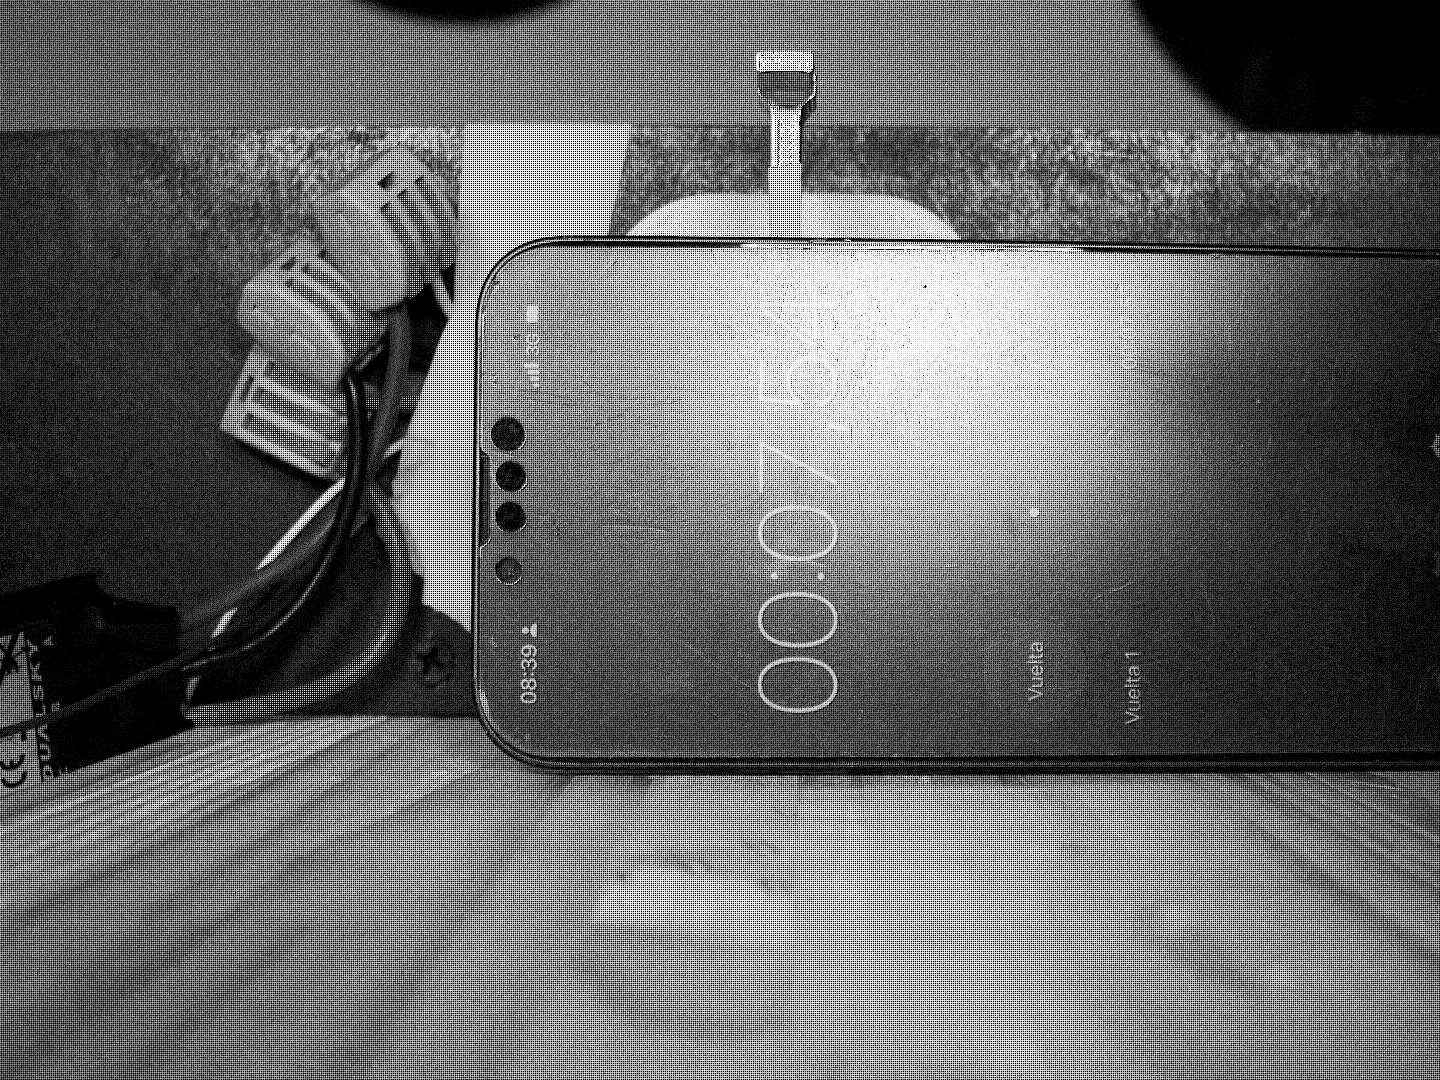
\includegraphics[width=0.8
    \textwidth]{FOTOS_C/1/0/3.png}
    \caption{Imagen 3 camara 0}
  \end{minipage}
  \begin{minipage}[b]{0.45\textwidth}
    \centering
    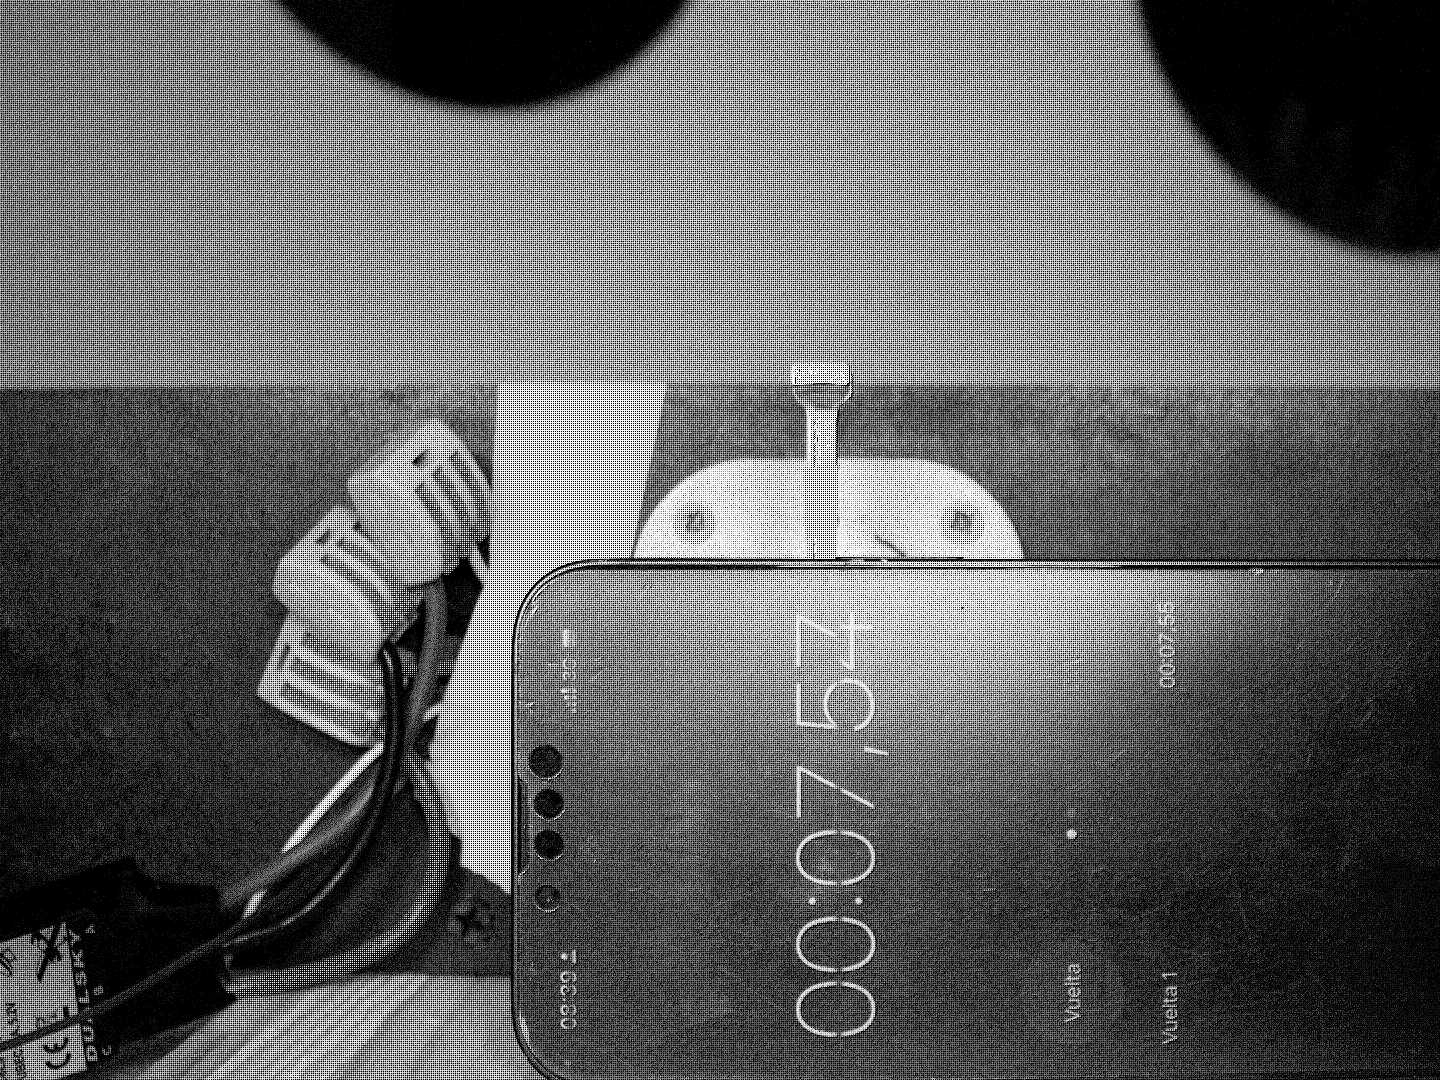
\includegraphics[width=0.8
    \textwidth]{FOTOS_C/1/1/3.png}
    \caption{Imagen 3 camara 1}
  \end{minipage}
  \begin{minipage}[b]{0.45\textwidth}
    \centering
    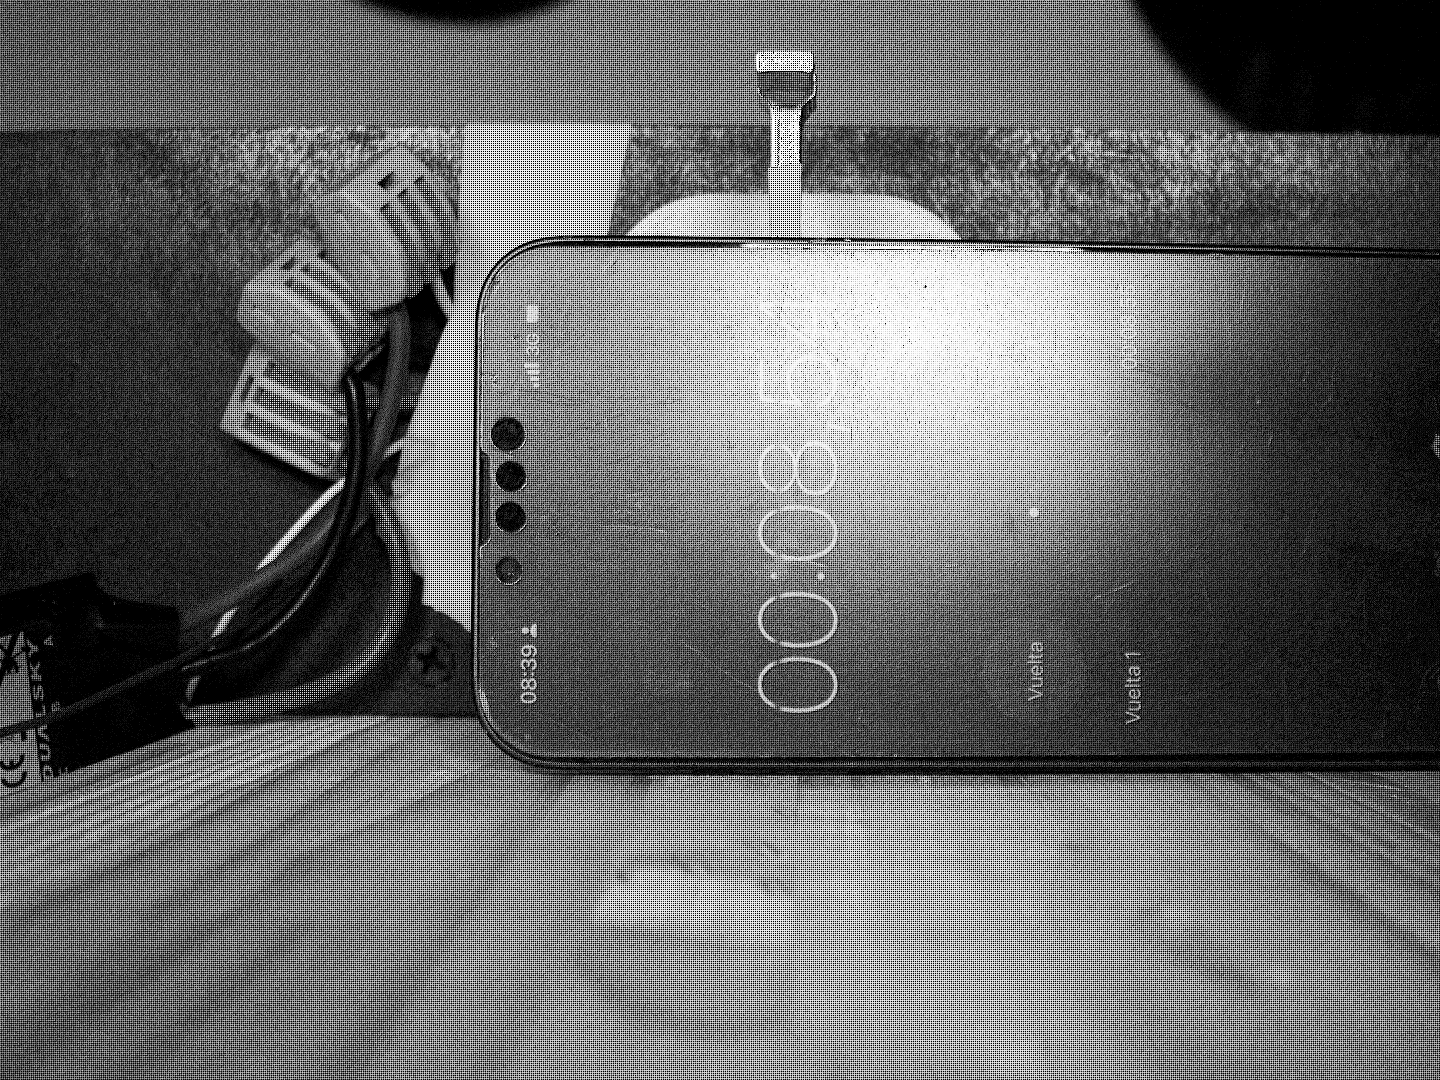
\includegraphics[width=0.8
    \textwidth]{FOTOS_C/1/0/4.png}
    \caption{Imagen 4 camara 0}
  \end{minipage}
  \begin{minipage}[b]{0.45\textwidth}
    \centering
    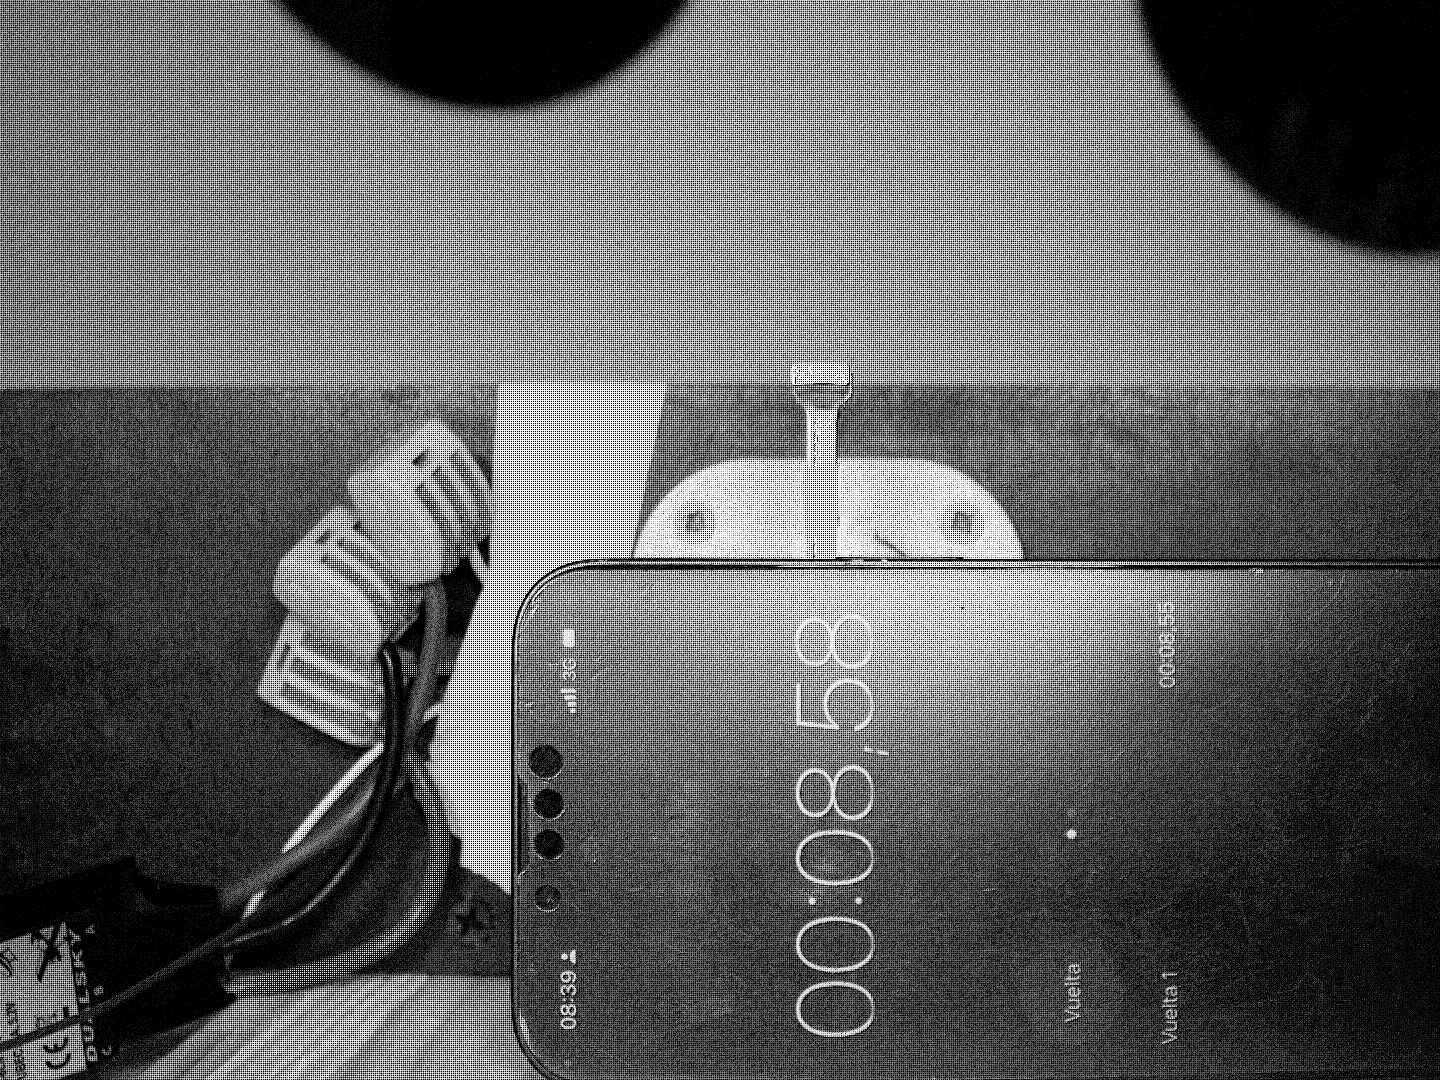
\includegraphics[width=0.8
    \textwidth]{FOTOS_C/1/1/4.png}
    \caption{Imagen 4 camara 1}
  \end{minipage}
\end{figure}

\newpage
\section {ANALISIS}

\noindent En primer lugar, surgió la incógnita de si el desfase era una pequeña porción de vuelta o una vuelta completa más fracción. Sin embargo, como se están sacando más fotos que RPS, significa que solo hay un desfase muy pequeño.
\\ \\
En base a lo anterior, y aproximando en grados, se obtiene lo siguiente:

\begin{center}
    \begin{tabular}{|c|c|}
    \hline
    RPM & DESFASE [s] \\
    \hline
    5645 & $1.6*10^{-5}$ \\
    \hline
    8519 & $3.4*10^{-5}$ \\
    \hline
    12055 & $3.9*10^{-5}$ \\
    \hline
    \end{tabular}
\end{center}

\noindent Una vez determinado que se logró la sincronización, se intentó sacar una gran cantidad de fotos, pero el programa tiene como límite 20, donde aún se desconoce la razón. Puede ser por la RAM, el software en sí mismo, etc. Aun así, el objetivo principal fue resuelto.

\section{CONCLUSION}
\noindent En conclusión, se logró sincronizar las cámaras con muy poco desfase, el cual siempre va a existir ya que el trigger es mediante SW, donde se corre un ciclo for. Si se hace mediante HW se podría erradicar esta diferencia, pero puede llegar a ser más costoso y complejo. Además, tomando a favor la velocidad del carbopol, se puede determinar que esta diferencia es despreciable en las mediciones.
\\ \\
Finalmente, se determinó que el próximo desafío es cómo tomar y procesar un gran número de fotos.

\newpage
\section{ESTRUCTURA CODIGO}

\noindent A continuación se mostrarán las partes clave del código. Primero se configuran las cámaras.

\begin{lstlisting}[language=Python]
  for i, cam in enumerate(cameras):
    cam.Attach(tlFactory.CreateDevice(devices[i]))

    cam.Open()
    cam.AcquisitionFrameRateEnable.SetValue(True)

    #Seteo FPS
    cam.AcquisitionFrameRate.SetValue(200)
    #Seteo exposicion
    cam.ExposureTime.SetValue(100) 
    cam.Close()
\end{lstlisting}

\noindent Posteriormente, se capturan las fotos, las cuales son guardadas inmediatamente en una lista en forma de array. De esta forma, se pierde el menor tiempo posible procesándolas.

\begin{lstlisting}[language=Python]
  for i in range(countOfImagesToGrab):
    if not cameras.IsGrabbing():
        break

    R = cameras.RetrieveResult(5000, pylon.TimeoutHandling_ThrowException)
    imagenes.append(R)
\end{lstlisting}

\noindent Finalmente, se procesan los arrays para obtener la imagen, el tiempo y la cámara que la tomó. De esta forma, es posible guardar las fotos de forma ordenada en sus respectivas carpetas.

\begin{lstlisting}[language=Python]
  for i, elementos in enumerate(imagenes):
    img = elementos.GetArray()
    img = cv2.equalizeHist(img)
    camara = elementos.GetCameraContext()
    tiempo = elementos.GetTimeStamp()

    folder_path = f'FOTOS/{RPM}/{camara}'
    print(folder_path)

    if not os.path.exists(folder_path):
        os.makedirs(folder_path)

    file_name = f'{tiempo}.png'

    file_path = os.path.join(folder_path, file_name)

    image = Image.fromarray(img)
    image.save(file_path)

    print(f"Imagen guardada: {file_path}")
\end{lstlisting}

\noindent Enlace a GitHub con toda la información: \href{https://github.com/LukasWolff2002/SINCRONIZACION_CAMARAS_BASLER}{GIT-HUB-INVESTIGACION-UHPC}.
\\ \\
\noindent Enlace a GitHub con codigo base: : \href{https://github.com/basler/pypylon/blob/master/samples/grabmultiplecameras.py}{GIT-HUB-CODIGO-BASE}.

\end{document}


